% ==============================================================================
% RELATÓRIO TÉCNICO — PRÁTICA 3: PROJETO DE FILTRO FIR PASSA-BAIXA (VERSÃO 02)
% Centro Universitário SENAI CIMATEC — Processamento Digital de Sinais (2026)
% Professor: Elio Pithon Sarno Filho
%
% Versão 02: texto revisado para seguir a notação e a linguagem das Aulas 12 a 17
% (M = ordem, K = M + 1 coeficientes, TFTD, tipos I a IV, buffer circular,
% formato Q, ruído de quantização Delta^2/12). Todos os valores numéricos
% vêm de results/ (gerados por src/main.m).
%
% INSTRUÇÕES DE COMPILAÇÃO NO OVERLEAF:
%   1. Crie um projeto em branco no Overleaf (Compilador: pdfLaTeX).
%   2. Faça upload deste arquivo na raiz do projeto.
%   3. Crie uma pasta `figures/` no Overleaf e envie os 8 arquivos `.pdf`
%      gerados pelo MATLAB na pasta `figures/` do repositório.
% ==============================================================================
\documentclass[11pt,a4paper]{article}

% --- Codificação, Fontes e Idioma ---
\usepackage[utf8]{inputenc}
\usepackage[T1]{fontenc}
\usepackage[brazilian]{babel}
\usepackage{lmodern}
\usepackage{microtype}
\usepackage{indentfirst}

% --- Geometria e Layout da Página ---
\usepackage[a4paper, top=2.2cm, bottom=2.2cm, left=2.0cm, right=2.0cm, headheight=15pt]{geometry}
\usepackage{fancyhdr}
\usepackage{titlesec}
\usepackage{enumitem}

% --- Matemática e Unidades ---
\usepackage{amsmath, amssymb, mathtools}
\usepackage{icomma} % vírgula decimal sem espaço extra em modo matemático
\usepackage{siunitx}
\sisetup{
    output-decimal-marker = {,},
    group-separator = {.},
    group-minimum-digits = 4,
    group-digits = integer,
    detect-all = true,
    per-mode = symbol
}

% --- Tabelas, Figuras e Cores ---
\usepackage{booktabs}
\usepackage{array}
\usepackage{tabularx}
\usepackage{multirow}
\usepackage{adjustbox}
\usepackage[table,xcdraw]{xcolor}
\usepackage{graphicx}
\graphicspath{{./figures/}{../figures/}{./}}
\usepackage{float}
\usepackage{caption}
\usepackage{subcaption}
\captionsetup{
    font=small,
    labelfont=bf,
    labelsep=period,
    justification=justified
}

% --- Diagramas Vetoriais (TikZ) ---
\usepackage{tikz}
\usetikzlibrary{arrows.meta, positioning, calc, shapes.geometric}

% --- Listagens de Código MATLAB ---
\usepackage{listings}

% Paleta institucional e de código
\definecolor{cimatecblue}{RGB}{0, 74, 143}
\definecolor{cimatecgray}{RGB}{242, 245, 249}
\definecolor{codebg}{RGB}{248, 249, 250}
\definecolor{codeframe}{RGB}{210, 215, 220}
\definecolor{codekw}{RGB}{0, 64, 150}
\definecolor{codecomment}{RGB}{34, 120, 55}
\definecolor{codestr}{RGB}{163, 21, 21}
\definecolor{rowpass}{RGB}{235, 248, 238}
\definecolor{rowfail}{RGB}{253, 242, 242}

\lstdefinestyle{matlabstyle}{
    language=Matlab,
    backgroundcolor=\color{codebg},
    frame=single,
    rulecolor=\color{codeframe},
    basicstyle=\ttfamily\footnotesize,
    keywordstyle=\color{codekw}\bfseries,
    commentstyle=\color{codecomment}\itshape,
    stringstyle=\color{codestr},
    numbers=left,
    numberstyle=\tiny\color{gray!80!black},
    stepnumber=1,
    numbersep=8pt,
    tabsize=4,
    showspaces=false,
    showstringspaces=false,
    breaklines=true,
    breakatwhitespace=true,
    captionpos=b,
     inputencoding=utf8,
    extendedchars=true,
    literate=%
        {á}{{\'a}}1 {é}{{\'e}}1 {í}{{\'i}}1 {ó}{{\'o}}1 {ú}{{\'u}}1
        {Á}{{\'A}}1 {É}{{\'E}}1 {Í}{{\'I}}1 {Ó}{{\'O}}1 {Ú}{{\'U}}1
        {à}{{\`a}}1 {ã}{{\~a}}1 {õ}{{\~o}}1 {â}{{\^a}}1 {ê}{{\^e}}1 {ô}{{\^o}}1
        {ç}{{\c{c}}}1 {Ç}{{\c{C}}}1
}

% --- Hiperlinks e Metadados do PDF ---
\usepackage[
    colorlinks=true,
    linkcolor=cimatecblue,
    citecolor=cimatecblue,
    urlcolor=cimatecblue,
    pdftitle={Prática 3 — Projeto de Filtro FIR Passa-Baixa (SENAI CIMATEC)},
    pdfauthor={Disciplina de Processamento Digital de Sinais — SENAI CIMATEC},
    pdfsubject={Projeto de Filtro FIR Passa-Baixa, Buffer Circular e Quantização em Ponto Fixo}
]{hyperref}

% --- Estilização de Seções e Cabeçalhos ---
\titleformat{\section}{\large\bfseries\color{cimatecblue}}{\thesection.}{0.5em}{}[\titlerule]
\titleformat{\subsection}{\normalsize\bfseries\color{cimatecblue!85!black}}{\thesubsection}{0.5em}{}
\titleformat{\subsubsection}{\normalsize\itshape\bfseries}{\thesubsubsection}{0.5em}{}
\titlespacing*{\section}{0pt}{14pt}{6pt}
\titlespacing*{\subsection}{0pt}{10pt}{4pt}
\titlespacing*{\subsubsection}{0pt}{8pt}{3pt}

\pagestyle{fancy}
\fancyhf{}
\fancyhead[L]{\footnotesize\textcolor{gray!80!black}{\textbf{SENAI CIMATEC} — Processamento Digital de Sinais}}
\fancyhead[R]{\footnotesize\textcolor{gray!80!black}{Prática 3: Projeto de Filtro FIR Passa-Baixa}}
\fancyfoot[C]{\footnotesize\thepage}
\renewcommand{\headrulewidth}{0.4pt}

% ==============================================================================
% MACROS OFICIAIS GERADAS AUTOMATICAMENTE POR src/main.m (results/metricas_relatorio.tex)
% Fonte única da verdade numérica para consistência com os scripts MATLAB
% ==============================================================================
% --- Etapa A: Projeto por Janelamento (Hamming) ---
\newcommand{\MetricaAN}{23}
\newcommand{\MetricaAOrdem}{22}
\newcommand{\MetricaADesvioPassdB}{0{,}042323}
\newcommand{\MetricaAAtenStopdB}{47{,}0065}
\newcommand{\MetricaASomaCoefs}{1{,}0000000000}
\newcommand{\MetricaAGanhoDCdB}{0{,}000000}
\newcommand{\MetricaAErroSimetria}{0{,}0000\times 10^{0}}
\newcommand{\MetricaAAtrasoAmostras}{11{,}0}
\newcommand{\MetricaAAtrasoMs}{1{,}3750}

% --- Etapa A2: Comparação com Equiripple ---
\newcommand{\MetricaAIIEqN}{15}
\newcommand{\MetricaAIIEqOrdem}{14}
\newcommand{\MetricaAIIEqDesvioPassdB}{0{,}083846}
\newcommand{\MetricaAIIEqAtenStopdB}{46{,}5690}
\newcommand{\MetricaAIIEqGanhoDCdB}{+0{,}082627}
\newcommand{\MetricaAIIEqSomaCoefs}{1{,}009558}
\newcommand{\MetricaAIIEqAtrasoAmostras}{7{,}0}
\newcommand{\MetricaAIIEqAtrasoMs}{0{,}8750}
\newcommand{\MetricaAIIReducaoCoefsPerc}{34{,}78}

% --- Etapa B: Buffer Circular ---
\newcommand{\MetricaBErroMaxImpFilter}{0{,}000000\times 10^{0}}
\newcommand{\MetricaBErroMaxImpH}{0{,}000000\times 10^{0}}
\newcommand{\MetricaBErroMaxSenFilter}{3{,}330669\times 10^{-16}}
\newcommand{\MetricaBGanhoPassLin}{0{,}99783632}
\newcommand{\MetricaBGanhoPassdB}{-0{,}018814}
\newcommand{\MetricaBGanhoStopLin}{0{,}00235009}
\newcommand{\MetricaBGanhoStopdB}{-52{,}5783}
\newcommand{\MetricaBAtenStopdB}{52{,}5783}

% --- Etapa C: Quantização de Coeficientes ---
\newcommand{\MetricaCErroMaxQXV}{1{,}397490\times 10^{-5}}
\newcommand{\MetricaCEQMQXV}{9{,}057312\times 10^{-11}}
\newcommand{\MetricaCSomaQXV}{0{,}99993896}
\newcommand{\MetricaCGanhoDCQXVdB}{-0{,}000530}
\newcommand{\MetricaCDesvioPassQXVdB}{0{,}042440}
\newcommand{\MetricaCAtenStopQXVdB}{46{,}9752}
\newcommand{\MetricaCErroMaxQVII}{2{,}673012\times 10^{-3}}
\newcommand{\MetricaCEQMQVII}{2{,}260906\times 10^{-6}}
\newcommand{\MetricaCSomaQVII}{0{,}97656250}
\newcommand{\MetricaCGanhoDCQVIIdB}{-0{,}205999}
\newcommand{\MetricaCDesvioPassQVIIdB}{0{,}205999}
\newcommand{\MetricaCAtenStopQVIIdB}{39{,}8632}

% --- Etapa D: Quantização de Amostras (Q1.7) ---
\newcommand{\MetricaDCasoISNRIn}{46{,}8120}
\newcommand{\MetricaDCasoISNROut}{55{,}8395}
\newcommand{\MetricaDCasoIDeltaSNR}{+9{,}0275}
\newcommand{\MetricaDCasoIISNRIn}{46{,}8428}
\newcommand{\MetricaDCasoIISNROut}{57{,}7056}
\newcommand{\MetricaDCasoIIDeltaSNR}{+10{,}8628}

% --- Etapa E: Precisão Aritmética e Overflow ---
\newcommand{\MetricaEProdCompleto}{0{,}21697998046875}
\newcommand{\MetricaEProdArred}{0{,}2187500}
\newcommand{\MetricaEErroArred}{+0{,}00177001953125}
\newcommand{\MetricaEProdTrunc}{0{,}2109375}
\newcommand{\MetricaEErroTrunc}{-0{,}00604248046875}
\newcommand{\MetricaENormaLI}{1{,}47339547500902}
\newcommand{\MetricaENormaLIdB}{3{,}3664}

% --- Métricas adicionadas após a Aula 18 (src/main.m executado no MATLAB Online em 27/11/2026) ---
\newcommand{\MetricaAErroFirI}{5{,}551115\times 10^{-17}}
\newcommand{\MetricaAAtrasoGdMedio}{11{,}000000}
\newcommand{\MetricaAAtrasoGdDesvio}{0{,}000000\times 10^{0}}
\newcommand{\MetricaCSomaAbsQXV}{1{,}47332764}
\newcommand{\MetricaCSomaAbsQVII}{1{,}47656250}
\newcommand{\MetricaEKMax}{86}
\newcommand{\MetricaEAMax}{0{,}671875}
\newcommand{\MetricaEPicoK}{126{,}7120}
\newcommand{\MetricaEPicoKI}{128{,}1854}
\newcommand{\MetricaEGanhoDCEsc}{0{,}678704}
\newcommand{\MetricaEGanhoDCEscdB}{-3{,}3664}
\newcommand{\MetricaESomaAbsEscQ}{1{,}0078125}
\newcommand{\MetricaESomaAbsEscQInt}{129}
\newcommand{\MetricaESomaEscQ}{0{,}6953125}
\newcommand{\MetricaESomaEscQInt}{89}
\newcommand{\MetricaEGanhoDCEscQdB}{-3{,}1564}
\newcommand{\MetricaEPicoEscQ}{0{,}9999390}
\newcommand{\MetricaEQRamo}{10}
\newcommand{\MetricaEQSoma}{9}
\newcommand{\MetricaEErroRamo}{0{,}08984375}
\newcommand{\MetricaEErroSoma}{0{,}00390625}


% --- Notação auxiliar ---
\newcommand{\sinc}{\operatorname{sinc}}

% ==============================================================================
\begin{document}

% --- CABEÇALHO INSTITUCIONAL SENAI CIMATEC ---
\noindent
\begin{tabular}{|p{0.62\textwidth}|p{0.32\textwidth}|}
    \hline
    \rowcolor{cimatecgray}
    \multicolumn{2}{|c|}{\vspace{2pt}\large\textbf{\textcolor{cimatecblue}{CENTRO UNIVERSITÁRIO SENAI CIMATEC}}\vspace{2pt}} \\
    \hline
    \textbf{Disciplina:} Processamento Digital de Sinais & \textbf{Avaliação:} Prática 3 \\
    \hline
    \textbf{Professor(a):} Elio Pithon Sarno Filho & \textbf{Data:} 02 de dezembro de 2026 \\
    \hline
    \textbf{Equipe:} Arthur Sant'Anna; Giulia Franca; Joseph Neiva; Matheus Sá & \textbf{Plataforma:} MATLAB R2026b \\
    \hline
\end{tabular}

\vspace{12pt}
\begin{center}
    {\LARGE\bfseries\textcolor{cimatecblue}{Projeto de Filtro FIR Passa-Baixa}}\\[4pt]
    {\normalsize Série de Fourier com janela de Hamming, filtragem com buffer circular e efeitos da precisão finita (\texttt{Q1.15} e \texttt{Q1.7})}
\end{center}
\vspace{4pt}

% ==============================================================================
% 1. OBJETIVO E ESPECIFICAÇÕES
% ==============================================================================
\section{Objetivo e Especificações do Filtro}

Esta prática tem como objetivo projetar um filtro digital FIR (\textit{Finite Impulse Response}) passa-baixa pelo método da série de Fourier com janelamento de Hamming, verificar a máscara de especificações, implementar a filtragem amostra por amostra com buffer circular e investigar, separadamente, os efeitos da precisão finita: quantização dos coeficientes, quantização das amostras e limites da aritmética de ponto fixo.

A escolha de um filtro FIR segue as diretrizes da Aula~12: por ser não recursivo, o FIR é \textbf{sempre estável}, permite garantir \textbf{fase linear} no projeto e é \textbf{menos sensível aos erros de precisão numérica finita} do que um IIR. O custo é um número maior de coeficientes para a mesma seletividade.

\paragraph{Notação.} Seguindo as aulas, $M$ é a \textbf{ordem} do filtro e $K = M + 1$ é o \textbf{número de coeficientes}. O roteiro e os scripts chamam o número de coeficientes de $N$ (tamanho do buffer em \texttt{fir\_circular}), portanto neste relatório $N \equiv K = M + 1$. Os coeficientes $b_k = h[k]$, $k = 0, 1, \dots, M$, definem a equação de diferenças e a função de transferência:
\begin{equation}
    y[n] = \sum_{k=0}^{M} b_k\, x[n-k], \qquad H(z) = \sum_{k=0}^{M} b_k\, z^{-k}, \qquad H(e^{j\omega}) = \sum_{k=0}^{M} b_k\, e^{-j\omega k}.
    \label{eq:fir}
\end{equation}

A Tabela~\ref{tab:especificacoes} reúne a máscara de especificações (\texttt{src/config\_specs.m}), também expressa em frequência normalizada $\omega = 2\pi f / F_s$ e em valores lineares de módulo.

\begin{table}[H]
    \centering
    \caption{Especificações do filtro FIR passa-baixa (máscara de projeto).}
    \label{tab:especificacoes}
    \small
    \begin{adjustbox}{max width=\textwidth}
    \begin{tabular}{@{}llll@{}}
        \toprule
        \textbf{Parâmetro} & \textbf{Símbolo (variável)} & \textbf{Valor} & \textbf{Equivalente normalizado / linear} \\
        \midrule
        Frequência de amostragem & $F_s$ (\texttt{Fs}) & \SI{8000}{Hz} & $T = 1/F_s = \SI{125}{\micro\second}$ \\
        Banda passante & $0 \le f \le F_{\text{pass}}$ (\texttt{Fpass}) & 0 a \SI{1000}{Hz} & $0 \le \omega \le \omega_p = 0,25\pi$ \\
        Desvio máximo na banda passante & \texttt{tol\_pass\_dB} & $\pm\SI{0,1}{dB}$ em torno de \SI{0}{dB} & $0,98855 \le |H| \le 1,01158$ \\
        Banda de rejeição & $F_{\text{stop}} \le f \le F_s/2$ (\texttt{Fstop}) & \SI{2200}{Hz} a \SI{4000}{Hz} & $\omega_s = 0,55\pi \le \omega \le \pi$ \\
        Atenuação mínima na rejeição & $A_{\min}$ (\texttt{aten\_stop\_dB}) & \SI{45}{dB} & $|H| \le 0,005623$ \\
        Banda de transição & $\Delta f = F_{\text{stop}} - F_{\text{pass}}$ & \SI{1000}{Hz} a \SI{2200}{Hz} ($\Delta f = \SI{1200}{Hz}$) & $\Delta\omega = 0,3\pi$ \\
        Frequência de corte ideal inicial & $f_c$ (\texttt{fc}) & \SI{1600}{Hz} (centro da transição) & $\omega_c = 0,4\pi$ \\
        Método principal & --- & Série de Fourier + janela de Hamming & --- \\
        Grade de avaliação da máscara & \texttt{Nfft} & \num{32768} pontos em $[0,\, F_s/2]$ & --- \\
        \bottomrule
    \end{tabular}
    \end{adjustbox}
\end{table}

% ==============================================================================
% 2. METODOLOGIA SUCINTA
% ==============================================================================
\section{Metodologia Sucinta}

O trabalho segue as cinco etapas do projeto de filtros digitais apresentadas na Aula~12, cada uma associada às etapas do roteiro. Todo o fluxo é executado sem intervenção manual por \texttt{src/main.m}, e todos os valores deste relatório foram lidos dos arquivos gerados em \texttt{results/}.

\begin{enumerate}[leftmargin=1.6em, itemsep=2pt, topsep=3pt]
    \item \textbf{Especificação:} máscara da Tabela~\ref{tab:especificacoes}.

    \item \textbf{Aproximação (Etapas A e A2):} cálculo dos coeficientes pelo \textbf{método direto}, típico de filtros FIR. Na Etapa~A, usa-se a série de Fourier com janela de Hamming, seguindo o procedimento de sete passos da Aula~15 (Seção~\ref{sec:etapaA}). Na Etapa~A2, o resultado é comparado com um projeto ótimo pelo algoritmo de Parks--McClellan (\textit{Equiripple}) feito no \textit{Filter Designer}. Todas as versões do filtro são avaliadas pela mesma rotina \texttt{avaliar\_mascara.m} (\texttt{freqz} com $N_{\text{FFT}} = \num{32768}$ pontos), que calcula o desvio máximo na passante e a atenuação mínima na rejeição.

    \item \textbf{Síntese e realização (Etapa B):} realização em \textbf{forma direta}, processada \textbf{amostra por amostra}, com o histórico de entrada mantido em um \textbf{buffer circular} (\texttt{fir\_circular}) e validação frente a \texttt{filter(h,1,x)}.

    \item \textbf{Análise de desempenho (Etapas C, D e E):} a Aula~17 classifica os efeitos da precisão finita em \textbf{erros de quantização} (dos coeficientes e das amostras do sinal) e \textbf{erros aritméticos} (arredondamento/truncamento e \textit{overflow}). Essas quatro situações são estudadas isoladamente: coeficientes em \texttt{Q1.15} e \texttt{Q1.7} com sinal e aritmética em ponto flutuante (Etapa~C); amostras de entrada em \texttt{Q1.7} com coeficientes em ponto flutuante (Etapa~D); e produto, arredondamento, truncamento, momento do arredondamento, amplitude máxima de entrada e \textit{overflow} em \texttt{Q1.7} (Etapa~E, conceitual, complementada pela Aula~18).

    \item \textbf{Implementação:} scripts MATLAB comentados, na pasta \texttt{src/}, e vetor final de coeficientes salvo no arquivo \texttt{coeficientes\_FIR.mat}, na pasta \texttt{data/}.
\end{enumerate}

% ==============================================================================
% 3. ETAPA A — PROJETO POR JANELAMENTO
% ==============================================================================
\section{Etapa A — Projeto por Janelamento (Série de Fourier + Hamming)}
\label{sec:etapaA}

\subsection{Procedimento de projeto}

O projeto aplica o procedimento da Aula~15 para filtros FIR por séries de Fourier e janelamento:

\begin{enumerate}[leftmargin=1.6em, itemsep=2pt, topsep=3pt]
    \item \textbf{Escolha da janela pela atenuação exigida na rejeição.} Na janela retangular, a relação entre o lóbulo principal e o primeiro lóbulo lateral é de apenas $\approx\SI{13,5}{dB}$, e o truncamento abrupto da resposta ideal causa o \textbf{fenômeno de Gibbs}: os \textit{ripples} de maior amplitude ficam na borda da transição e não diminuem com a ordem. Na janela de Hamming, essa relação é de $\approx\SI{42}{dB}$, e o filtro resultante tem atenuação de pico na rejeição da ordem de \SI{53}{dB} (Oppenheim). A janela de Hamming é, portanto, compatível com os \SI{45}{dB} exigidos.

    \item \textbf{Tamanho da janela pela largura de transição.} A transição especificada é
    \begin{equation}
        \Delta f = F_{\text{stop}} - F_{\text{pass}} = \SI{1200}{Hz}, \qquad \Delta\omega = \frac{2\pi\,\Delta f}{F_s} = 0,3\pi \approx \SI{0,942478}{rad/amostra}.
    \end{equation}
    Para a janela de Hamming, a relação aproximada entre largura de transição e comprimento é $\Delta\omega \approx 6,6\pi/N$, ou seja, $\Delta f/F_s \approx 3,3/N$:
    \begin{equation}
        N_{\text{est}} = \left\lceil \frac{3,3}{\Delta f / F_s} \right\rceil = \left\lceil \frac{3,3}{0,15} \right\rceil = 22 \text{ coeficientes } (M = 21).
    \end{equation}
    Como referência conservadora, igualar $\Delta\omega$ à largura total do lóbulo principal da janela ($8\pi/N$) leva a $N_{\text{est,alt}} = \lceil 4,0/0,15 \rceil = 27$ ($M = 26$).

    \item \textbf{Coeficientes da janela de Hamming} de comprimento $N$: $w[n] = 0,54 - 0,46\cos\!\left(\dfrac{2\pi n}{N-1}\right) = 0,54 - 0,46\cos\!\left(\dfrac{2\pi n}{M}\right)$, $n = 0, 1, \dots, M$ (no MATLAB, \texttt{hamming(N)}).

    \item \textbf{Resposta impulsiva ideal} do passa-baixa, pela transformada inversa (TFTD inversa) da resposta desejada: $h[n] = \dfrac{\omega_c}{\pi}\sinc\!\left(\dfrac{\omega_c n}{\pi}\right)$, bilateral e de comprimento infinito.

    \item[5--6.] \textbf{Truncamento e deslocamento causal.} Mantém-se apenas $-M/2 \le n \le M/2$ e desloca-se a sequência $M/2$ amostras para a direita, obtendo-se os coeficientes $b'_k$ centrados em $M/2 = (N-1)/2$:
    \begin{equation}
        b'_k = \frac{\omega_c}{\pi}\,\sinc\!\left(\frac{\omega_c\,(k - M/2)}{\pi}\right) = 0,4\,\sinc\big(0,4\,(k - M/2)\big), \qquad k = 0, 1, \dots, M.
        \label{eq:hideal}
    \end{equation}
    Na forma $\sin(\cdot)/(\cdot)$ usada no script, o termo central $k = M/2$ (que existe quando $N$ é ímpar) é tratado explicitamente como $b'_{M/2} = \omega_c/\pi = 0,4$, evitando a indeterminação $0/0$.

    \item[7.] \textbf{Janelamento e normalização:} $b_k = b'_k\,w[k]$, seguido da normalização pedida no roteiro (\texttt{h = h/sum(h)}):
    \begin{equation}
        h[k] = \frac{b'_k\,w[k]}{\sum_{i=0}^{M} b'_i\,w[i]}, \qquad k = 0, 1, \dots, M.
        \label{eq:hnorm}
    \end{equation}
\end{enumerate}

\subsection{Comprimentos testados e filtro selecionado}

Como a estimativa é apenas aproximada, foram testados todos os comprimentos, pares e ímpares, de $N = 15$ a $45$. A Tabela~\ref{tab:A1_varredura} mostra os resultados de $N = 15$ a $31$. A coluna ``Tipo'' segue a classificação da Aula~14: com coeficientes simétricos, $N$ ímpar ($M$ par) gera filtro do \textbf{tipo~I} e $N$ par ($M$ ímpar) gera filtro do \textbf{tipo~II}.

\begin{table}[H]
    \centering
    \caption{Comprimentos testados (série de Fourier + Hamming, $f_c = \SI{1600}{Hz}$), incluindo os que falharam (\texttt{results/tab\_A1\_varredura\_N.csv}). Em verde, o menor comprimento que atende à máscara.}
    \label{tab:A1_varredura}
    \footnotesize
    \setlength{\tabcolsep}{5pt}
    \begin{adjustbox}{max width=\textwidth}
    \begin{tabular}{@{}cccSSccc@{}}
        \toprule
        \textbf{$N = K$} & \textbf{Ordem $M$} & \textbf{Tipo} & {\textbf{Desvio pass.\ máx.\ [\si{dB}]}} & {\textbf{Aten.\ rej.\ mín.\ [\si{dB}]}} & \textbf{Passante?} & \textbf{Rejeição?} & \textbf{Máscara?} \\
        & & & {($\le 0,1$)} & {($\ge 45$)} & & & \\
        \midrule
        15 & 14 & I  & 0.615336 & 23.2696 & Não & Não & Não \\
        16 & 15 & II & 0.472802 & 25.5998 & Não & Não & Não \\
        17 & 16 & I  & 0.359812 & 28.0554 & Não & Não & Não \\
        18 & 17 & II & 0.264299 & 30.1168 & Não & Não & Não \\
        19 & 18 & I  & 0.179714 & 32.4023 & Não & Não & Não \\
        20 & 19 & II & 0.109923 & 35.9892 & Não & Não & Não \\
        \rowcolor{rowfail}
        21 & 20 & I  & 0.063688 & 40.6091 & Sim & \textbf{Não} & \textbf{Não} \\
        \rowcolor{rowfail}
        22 ($N_{\text{est}}$) & 21 & II & 0.044035 & 44.0615 & Sim & \textbf{Não} & \textbf{Não} \\
        \rowcolor{rowpass}
        \textbf{23} & \textbf{22} & \textbf{I} & \textbf{0,042323} & \textbf{47,0065} & \textbf{Sim} & \textbf{Sim} & \textbf{Sim (escolhido)} \\
        24 & 23 & II & 0.046770 & 49.8082 & Sim & Sim & Sim \\
        25 & 24 & I  & 0.049449 & 50.1908 & Sim & Sim & Sim \\
        26 & 25 & II & 0.034964 & 53.5795 & Sim & Sim & Sim \\
        27 ($N_{\text{est,alt}}$) & 26 & I & 0.019279 & 53.0635 & Sim & Sim & Sim \\
        28 & 27 & II & 0.037329 & 52.2583 & Sim & Sim & Sim \\
        29 & 28 & I  & 0.043283 & 50.7077 & Sim & Sim & Sim \\
        30 & 29 & II & 0.044155 & 51.3627 & Sim & Sim & Sim \\
        31 & 30 & I  & 0.032945 & 56.8528 & Sim & Sim & Sim \\
        \midrule
        \multicolumn{8}{@{}p{0.94\textwidth}@{}}{\scriptsize \textit{Nota:} todos os comprimentos de $N = 32$ a $45$ também atendem à máscara (desvio entre \SI{0,011246}{dB} e \SI{0,039526}{dB}; atenuação entre \SI{53,0889}{dB} e \SI{62,2523}{dB}). Após a normalização, o ganho DC é \SI{0}{dB} em todos os casos (resíduo numérico $< \num{6e-15}$~dB).} \\
        \bottomrule
    \end{tabular}
    \end{adjustbox}
\end{table}

O filtro escolhido ($N = \MetricaAN$, salvo em \texttt{data/coeficientes\_FIR.mat}) está resumido na Tabela~\ref{tab:A2_metricas}. A Figura~\ref{fig:A1_impulso} mostra a resposta impulsiva ideal, a janela e os coeficientes finais, e a Figura~\ref{fig:A2_magnitude} mostra a magnitude com os limites da máscara.

\begin{table}[H]
    \centering
    \caption{Resultados do filtro selecionado na Etapa A.}
    \label{tab:A2_metricas}
    \small
    \begin{tabular}{@{}lcl@{}}
        \toprule
        \textbf{Grandeza} & \textbf{Valor} & \textbf{Observação} \\
        \midrule
        Número de coeficientes $N = K$ & $\MetricaAN$ & tipo I (simétrico, $K$ ímpar) \\
        Ordem $M = N - 1$ & $\MetricaAOrdem$ & --- \\
        Desvio máximo na passante (\SIrange{0}{1000}{Hz}) & $\MetricaADesvioPassdB$~\si{dB} & limite $\le \SI{0,1}{dB}$: atende \\
        Atenuação mínima na rejeição (\SIrange{2200}{4000}{Hz}) & $\MetricaAAtenStopdB$~\si{dB} & limite $\ge \SI{45}{dB}$: atende \\
        Soma dos coeficientes $\sum_k h[k]$ & $\MetricaASomaCoefs$ & ganho DC $= $\MetricaAGanhoDCdB$~\si{dB}$ \\
        Erro máximo de simetria $\max_k |h[k] - h[M-k]|$ & $0$ & simetria exata \\
        Atraso de grupo $\tau_g = M/2$ & $\MetricaAAtrasoAmostras$~\si{amostras} & $= $\MetricaAAtrasoMs$~\si{ms}$ \\
        \bottomrule
    \end{tabular}
\end{table}

\begin{figure}[H]
    \centering
    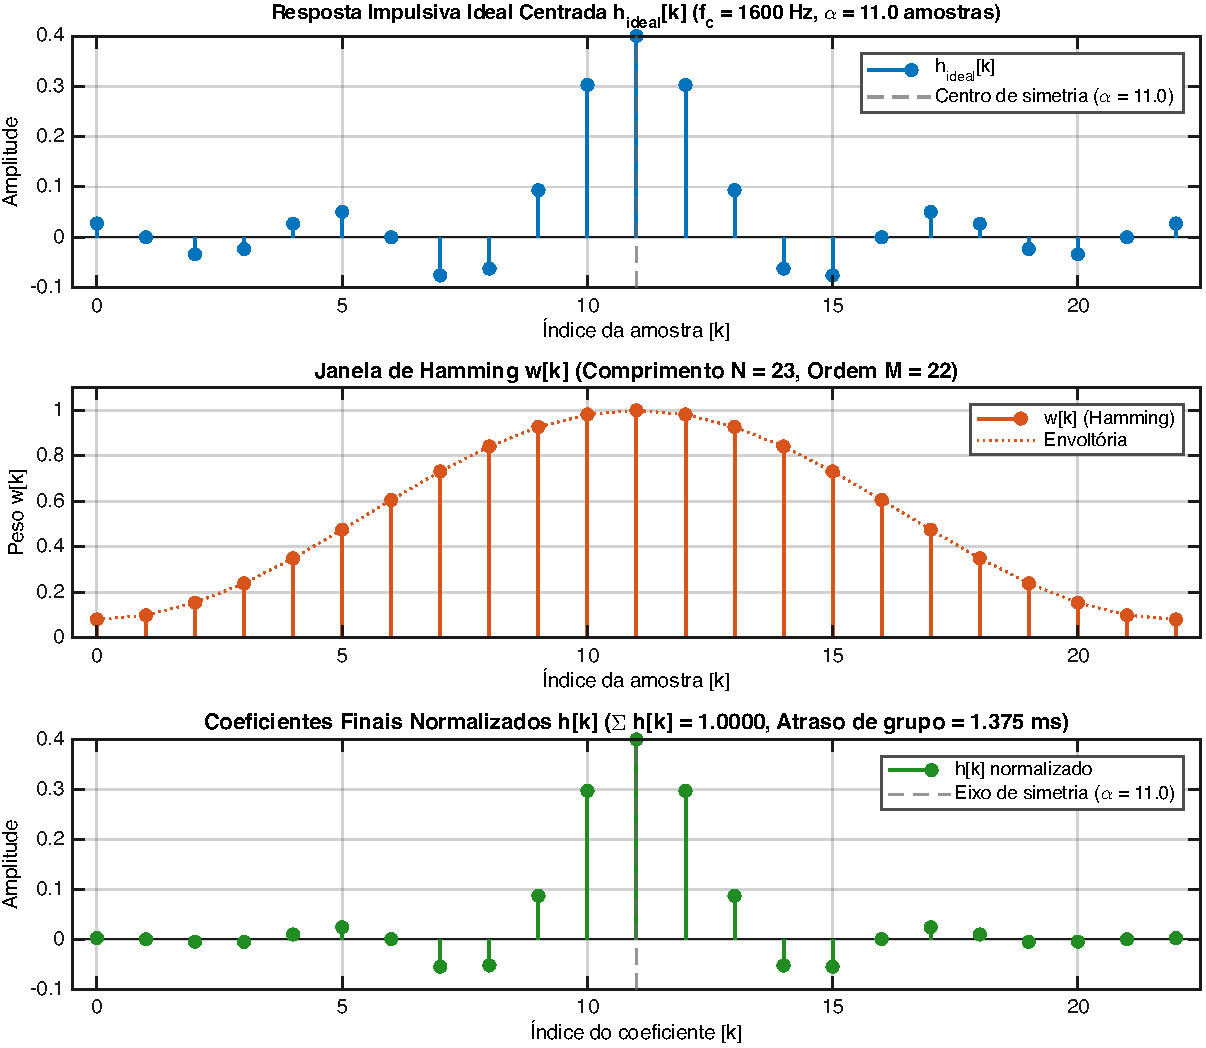
\includegraphics[width=0.92\linewidth]{fig_A1_impulso_janela.pdf}
    \caption{Etapa A: resposta impulsiva ideal truncada e deslocada ($b'_k$, centrada em $M/2 = 11$), janela de Hamming $w[k]$ com $N = 23$ e coeficientes finais normalizados $h[k]$.}
    \label{fig:A1_impulso}
\end{figure}

\begin{figure}[H]
    \centering
    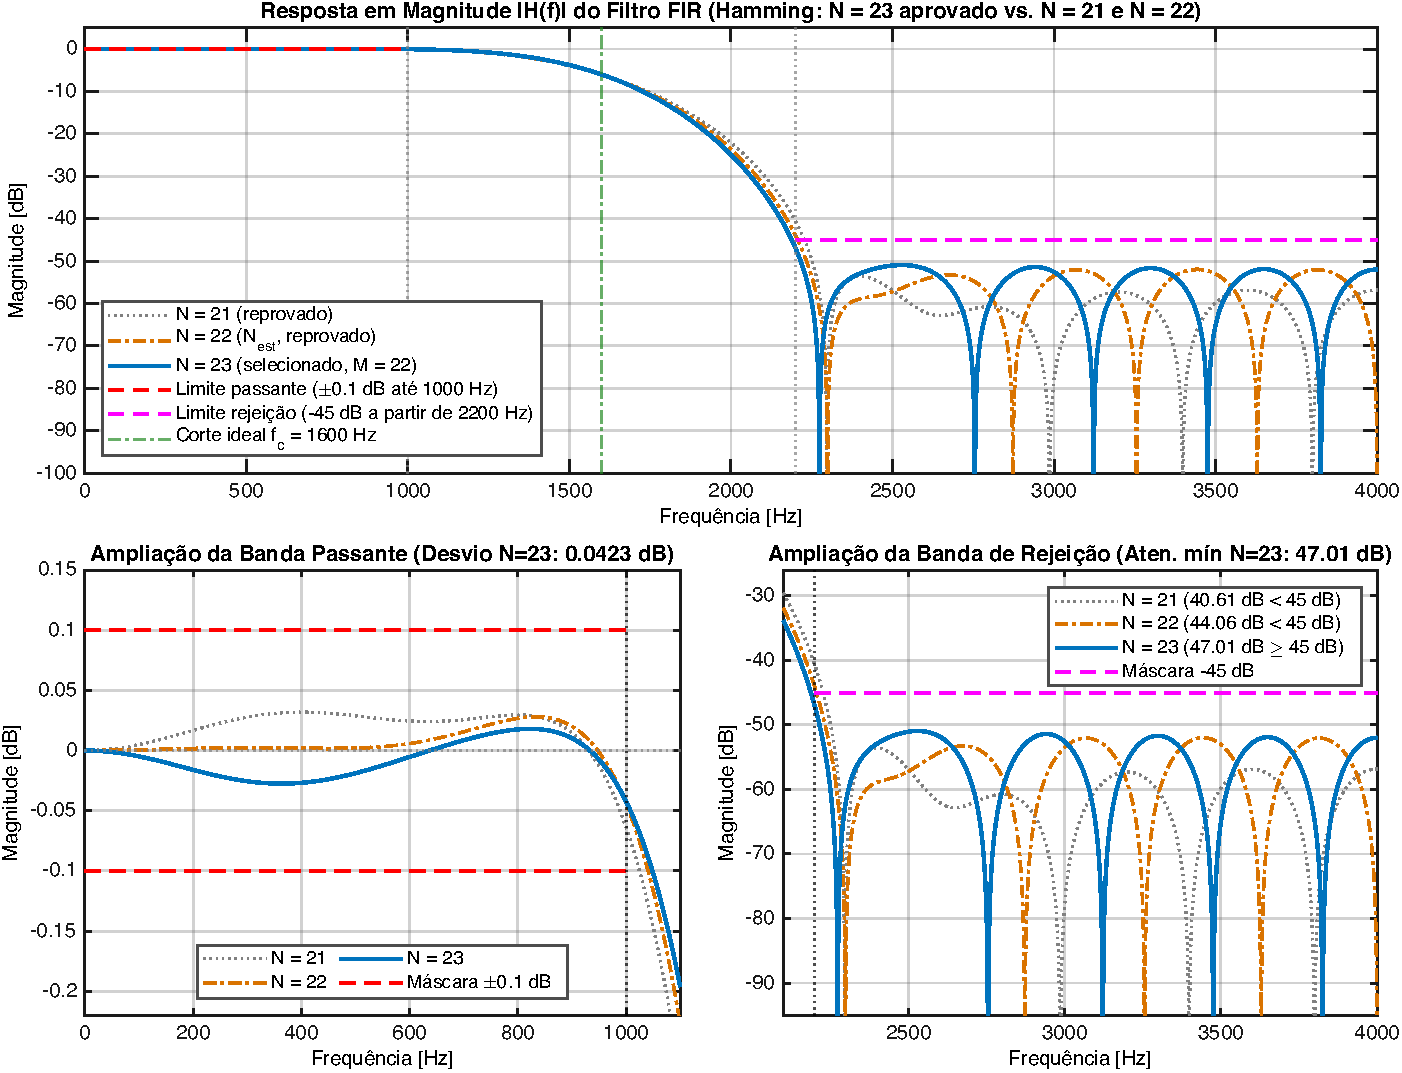
\includegraphics[width=0.96\linewidth]{fig_A2_magnitude_mascara.pdf}
    \caption{Etapa A: magnitude $|H(f)|$ em dB de \SI{0}{Hz} a \SI{4000}{Hz} para $N = 23$ e para os candidatos reprovados $N = 21$ e $N = 22$, com os limites da máscara e ampliações da banda passante ($\pm\SI{0,1}{dB}$) e da banda de rejeição ($-\SI{45}{dB}$).}
    \label{fig:A2_magnitude}
\end{figure}

\subsection{Análise (Etapa A)}

\begin{itemize}[leftmargin=1.5em, itemsep=3pt]
    \item \textbf{Estimativa de ordem $\times$ verificação efetiva da máscara.} A relação $\Delta f/F_s \approx 3,3/N$ descreve apenas a largura típica da transição da janela de Hamming. Ela não leva em conta os níveis exatos de \SI{0,1}{dB} em \SI{1000}{Hz} e de \SI{45}{dB} a partir de \SI{2200}{Hz}, nem o valor fixo $f_c = \SI{1600}{Hz}$. Por isso a estimativa serve só como ponto de partida, e o cumprimento da máscara precisa ser verificado. A Tabela~\ref{tab:A1_varredura} confirma isso: $N = 22$ atende à passante (\SI{0,044035}{dB}) mas falha na rejeição (\SI{44,0615}{dB} $< \SI{45}{dB}$), e o mesmo acontece com $N = 21$.

    \item \textbf{Justificativa de $N = 23$.} Com $N = 23$ ($M = 22$), o lóbulo principal fica mais estreito e a transição mais abrupta, de modo que a atenuação mínima chega a \SI{47,0065}{dB}, com desvio na passante de \SI{0,042323}{dB}. Este é o menor comprimento testado que atende às duas exigências. Comprimentos maiores também atendem, mas aumentam o número de multiplicações por amostra e o atraso de grupo. Isso reproduz o compromisso da Aula~14: menores ondulações, maior atenuação e transição mais estreita exigem uma ordem $M$ maior.

    \item \textbf{Função da normalização.} Fazendo $\omega = 0$ na Equação~\eqref{eq:fir}, obtém-se $H(e^{j0}) = \sum_k h[k]$: o \textbf{ganho DC é a soma dos coeficientes}. Após o truncamento e o janelamento, $\sum_k b'_k w[k]$ fica um pouco diferente de 1. A divisão da Equação~\eqref{eq:hnorm} impõe soma unitária (\MetricaASomaCoefs) e ganho DC de \SI{0}{dB}. Como todos os coeficientes são multiplicados pelo mesmo fator positivo, a forma relativa da resposta, as posições dos zeros e a fase não mudam (Aula~17). A normalização, por si só, não garante que toda a banda passante atenda à máscara: isso continua sendo verificado em \texttt{avaliar\_mascara.m}.

    \item \textbf{Simetria e fase linear.} A resposta ideal ($h[-n] = h[n]$) e a janela de Hamming são simétricas em torno de $M/2$, logo $h[k] = h[M-k]$ (erro de simetria nulo). Com $M$ par, separando o termo central e agrupando os pares $k$ e $M - k$ (Aula~13):
    \begin{equation}
        H(e^{j\omega}) = e^{-j\omega M/2}\, \underbrace{\left[\, h[M/2] + 2\sum_{k=0}^{M/2-1} h[k]\cos\!\Big(\omega\big(\tfrac{M}{2} - k\big)\Big) \right]}_{A(\omega)\,\in\,\mathbb{R}}.
    \end{equation}
    Como $A(\omega)$ é real, a fase é $\phi(\omega) = -\omega M/2 = -11\omega$ nos intervalos em que $A(\omega) > 0$, com saltos de $\pi$ ($180^\circ$) onde $A(\omega)$ muda de sinal, o que ocorre nos zeros da banda de rejeição. A fase é, portanto, \textbf{linear por trechos com a mesma inclinação}, e o atraso de grupo é constante: $\tau_g = M/2 = \SI{11}{amostras} = \SI{1,375}{ms}$. Todas as componentes da banda passante são atrasadas pelo mesmo tempo, sem distorção de fase. Os comprimentos pares testados (tipo~II) também têm fase linear, mas com atraso semi-inteiro ($M/2 = 10,5$ para $N = 22$), o que não exige atrasadores de meia amostra.

    \item \textbf{Conferência com as ferramentas do MATLAB.} A Aula~18 sugere usar \texttt{fir1} e \texttt{hamming} como referência para o projeto por série de Fourier e janelamento, e \texttt{grpdelay} para conferir o atraso de $M/2$ amostras. O comando \texttt{fir1(22, 0.4, hamming(23))}, que também normaliza o ganho DC para 1, gerou coeficientes que diferem de $h[k]$ em no máximo $\MetricaAErroFirI$. O atraso de grupo medido na banda passante foi de $\MetricaAAtrasoGdMedio$~amostras, com desvio máximo de $\MetricaAAtrasoGdDesvio$~amostras em relação a $M/2 = 11$.
\end{itemize}

% ==============================================================================
% 4. ETAPA A2 — FILTER DESIGNER
% ==============================================================================
\section{Etapa A2 — Filter Designer como Ferramenta Auxiliar}

Os coeficientes do janelamento ($N = 23$) foram analisados no \textit{Filter Designer} ($F_s = \SI{8000}{Hz}$), onde se conferiram a magnitude, a fase linear, o atraso de grupo constante de 11 amostras e o diagrama de zeros, em concordância com os gráficos do script.

Em seguida, criou-se no \textit{Filter Designer} um segundo FIR passa-baixa, com a mesma máscara, pelo método \textit{Equiripple} de ordem mínima. Seguindo o roteiro de uso da Aula~18, foram escolhidos: \textit{Response} = \textit{Lowpass}, tipo FIR; unidades em \si{Hz} com $F_s = \SI{8000}{Hz}$; \textit{Filter Order} = \textit{Minimum}; \textit{Passband and stopband frequencies}, com $F_{\text{pass}} = \SI{1000}{Hz}$ e $F_{\text{stop}} = \SI{2200}{Hz}$; \textit{Passband ripple} = \SI{0,2}{dB}, que corresponde à oscilação pico a pico de $\pm\SI{0,1}{dB}$; \textit{Stopband attenuation} = \SI{45}{dB}; e algoritmo \textit{Equiripple}, com fase linear. Esse método usa o algoritmo de \textbf{Parks--McClellan}, que emprega o algoritmo de troca de Remez e a aproximação de Chebyshev para \textbf{distribuir o erro máximo entre as frequências extremas} (Aula~15; em linha de comando, \texttt{b = firpm(M,f,m)}). Os coeficientes foram exportados por \textit{Export} $\to$ \textit{Export to MATLAB Workspace} $\to$ \textit{Coefficients} (o vetor recebe o sufixo \texttt{\_Num}), salvos em \texttt{data/coeficientes\_equiripple.mat} e avaliados pela mesma rotina \texttt{avaliar\_mascara.m}. Esse filtro é \textbf{apenas uma referência comparativa}: as Etapas B a E usam somente o filtro do janelamento.

\begin{table}[H]
    \centering
    \caption{Comparação entre o projeto por janelamento (Hamming) e o \textit{Equiripple} de ordem mínima (\texttt{results/tab\_A2\_comparacao\_equiripple.csv}).}
    \label{tab:A2_equiripple}
    \small
    \begin{adjustbox}{max width=\textwidth}
    \begin{tabular}{@{}lcc@{}}
        \toprule
        \textbf{Resultado} & \textbf{Janelamento} & \textbf{Equiripple} \\
        \midrule
        \textbf{Número de coeficientes} & $\mathbf{\MetricaAN}$ ($M = \MetricaAOrdem$) & $\mathbf{\MetricaAIIEqN}$ ($M = \MetricaAIIEqOrdem$) \\
        \textbf{Desvio máximo na passante [\si{dB}]} & $\mathbf{\MetricaADesvioPassdB}$ & $\mathbf{\MetricaAIIEqDesvioPassdB}$ \\
        \textbf{Atenuação mínima na rejeição [\si{dB}]} & $\mathbf{\MetricaAAtenStopdB}$ & $\mathbf{\MetricaAIIEqAtenStopdB}$ \\
        \textbf{Atende à máscara?} & \textbf{Sim} & \textbf{Sim} \\
        \midrule
        Ganho DC [\si{dB}] (soma dos coeficientes) & $\MetricaAGanhoDCdB$ ($1,000000$) & $\MetricaAIIEqGanhoDCdB$ ($\MetricaAIIEqSomaCoefs$) \\
        Atraso de grupo $M/2$ & $\MetricaAAtrasoAmostras$~\si{amostras} ($\MetricaAAtrasoMs$~\si{ms}) & $\MetricaAIIEqAtrasoAmostras$~\si{amostras} ($\MetricaAIIEqAtrasoMs$~\si{ms}) \\
        Multiplicações por amostra --- forma direta & 23 & 15 \\
        Multiplicações por amostra --- explorando a simetria & 12 & 8 \\
        Multiplicações por segundo (forma direta, $F_s = \SI{8000}{Hz}$) & \num{184000} & \num{120000} ($-\SI{34,78}{\percent}$) \\
        \bottomrule
    \end{tabular}
    \end{adjustbox}
\end{table}

\begin{figure}[H]
    \centering
    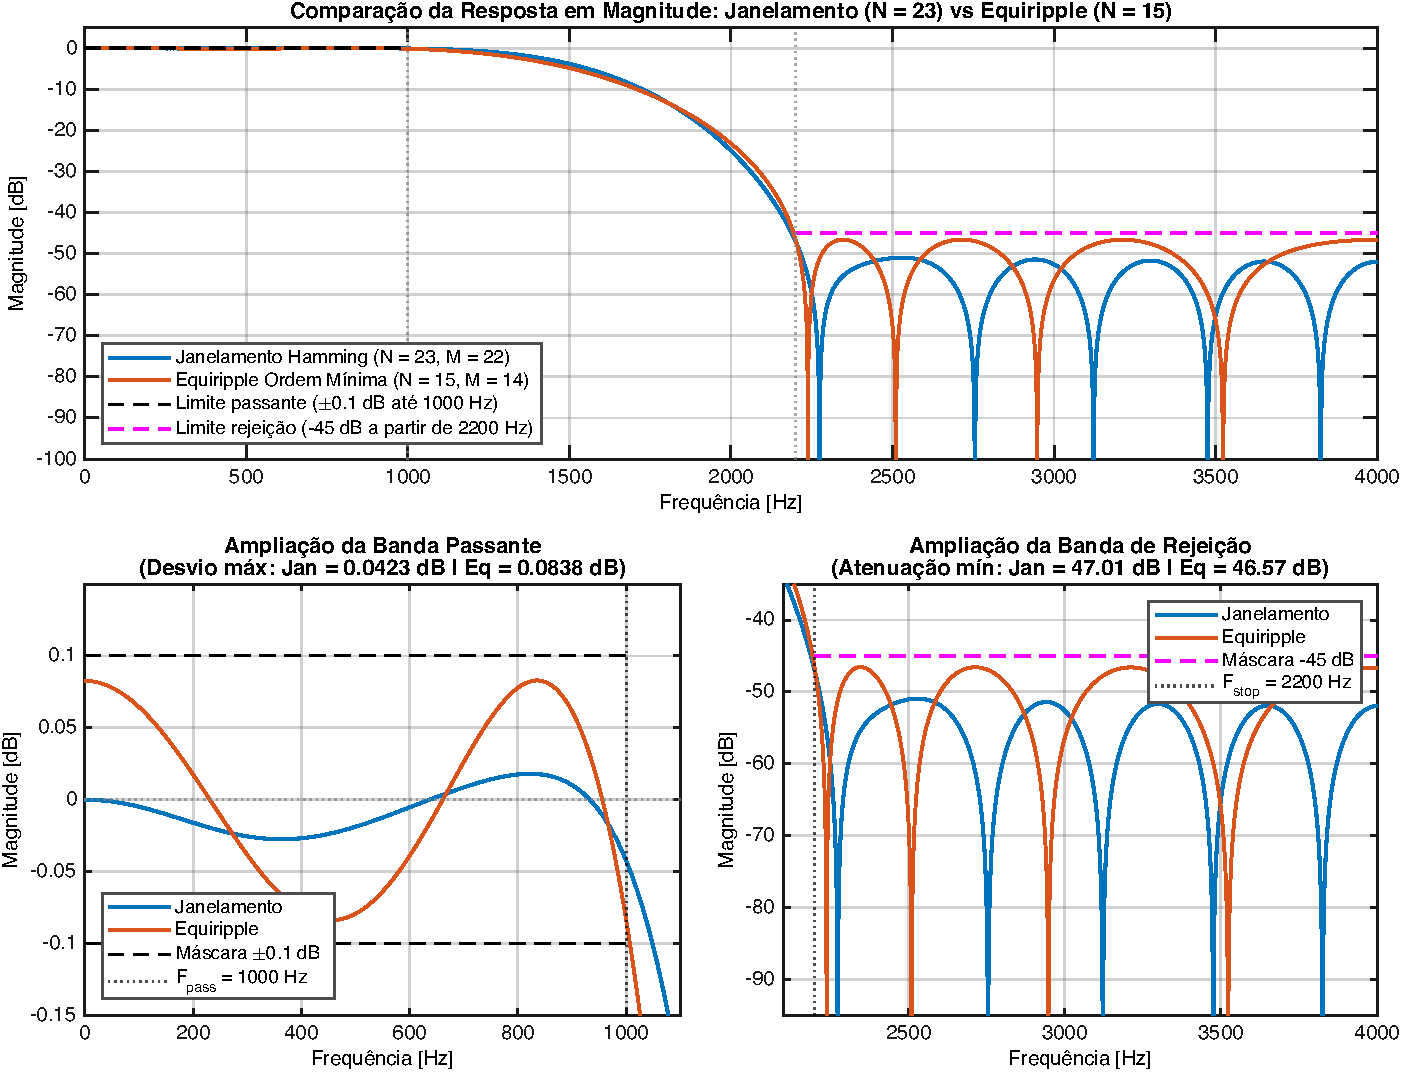
\includegraphics[width=0.96\linewidth]{fig_A2_comp_janelamento_equiripple.pdf}
    \caption{Etapa A2: magnitudes do filtro por janelamento de Hamming ($N = 23$) e do \textit{Equiripple} de ordem mínima ($N = 15$), com ampliações das bandas passante e de rejeição.}
    \label{fig:A2_comp_eq}
\end{figure}

\paragraph{Discussão: número de coeficientes, método de projeto e custo computacional.}
No janelamento, os coeficientes são o produto direto da resposta ideal pela janela. O erro fica concentrado perto da transição e diminui longe dela (Figura~\ref{fig:A2_comp_eq}): a passante fica bem abaixo do limite de \SI{0,1}{dB} na maior parte da banda, e os lóbulos da rejeição decaem para longe de \SI{2200}{Hz}. Em outras palavras, o filtro sobra em especificação no interior das bandas para conseguir atender às bordas. O \textit{Equiripple} distribui o erro de forma uniforme: as ondulações têm a mesma amplitude em toda a passante (desvio de \SI{0,083846}{dB}, inclusive em DC, \SI{+0,082627}{dB}) e em toda a rejeição (\SI{46,5690}{dB}). Por aproveitar melhor a tolerância da máscara, ele precisa de menos coeficientes: 15 contra 23.

O custo computacional acompanha o número de coeficientes. Na forma direta, cada saída exige $N$ multiplicações e $N - 1$ somas, ou seja, uma redução de \SI{34,78}{\percent} no número de multiplicações por segundo. Explorando a simetria (Aula~14), as amostras $x[n-k]$ e $x[n-M+k]$ são somadas antes da multiplicação pelo coeficiente comum, e o número de multiplicações cai para $\lceil N/2 \rceil$: 12 contra 8. A memória do buffer também diminui (15 contra 23 posições), e o atraso de grupo cai de \SI{1,375}{ms} para \SI{0,875}{ms}. O preço do \textit{Equiripple} é um ganho DC diferente de \SI{0}{dB} (dentro da tolerância) e um projeto iterativo, em vez de uma fórmula fechada.

% ==============================================================================
% 5. ETAPA B — BUFFER CIRCULAR
% ==============================================================================
\section{Etapa B — Implementação com Buffer Circular (\texttt{fir\_circular})}

\subsection{Realização e trecho essencial do código}

A função \texttt{fir\_circular(x,h)} realiza a forma direta da Equação~\eqref{eq:fir} \textbf{amostra por amostra}: a cada nova entrada $x[n]$, calcula $y[n]$ com a amostra atual e as $M$ anteriores, guardadas no buffer. Em tempo real, os $N = 23$ produtos precisam ser concluídos dentro de um período de amostragem ($T = \SI{125}{\micro\second}$). A função não chama \texttt{filter}, \texttt{conv} nem \texttt{fftfilt}.

A convenção é a das Aulas~14 e~16: as posições do buffer são numeradas no sentido horário; o ponteiro da amostra mais recente (\texttt{idx\_recente}) é \textbf{atualizado no sentido anti-horário}, e a nova amostra é escrita sobre a mais antiga; a leitura parte da amostra mais recente e percorre o buffer no \textbf{sentido horário} com um índice auxiliar separado (\texttt{idx\_leitura}). No MATLAB, os índices começam em 1, então o coeficiente \texttt{h(k)}, $k = 1, \dots, N$, corresponde a $b_{k-1}$, e o laço calcula $y[n] = \sum_{k=1}^{N} h(k)\,x[n-k+1]$.

\begin{lstlisting}[style=matlabstyle, caption={Trecho essencial de \texttt{src/fir\_circular.m}.}, label={lst:fir_circular}]
buf = zeros(1, N);             % Buffer circular de N amostras inicializado em repouso [amplitude]
y_lin = zeros(1, num_amostras);% Pre-alocacao do vetor de saida [amplitude]
idx_recente = 1;               % Ponteiro para a amostra mais recente no buffer (1..N) [indice]

for n = 1:num_amostras
    % Escrita: ponteiro avanca no sentido anti-horario e sobrescreve a amostra mais antiga
    idx_recente = idx_recente - 1;
    if idx_recente < 1
        idx_recente = N;           % Retorno circular ao final do anel
    end
    buf(idx_recente) = x_lin(n);   % Armazena a nova amostra x(n) [amplitude]

    % Leitura: indice auxiliar percorre o buffer no sentido horario a partir de idx_recente
    idx_leitura = idx_recente;
    acumulador  = 0.0;             % Acumulador da soma de produtos [amplitude]
    for k = 1:N
        acumulador = acumulador + h_lin(k) * buf(idx_leitura); % h(k) * x(n - k + 1)
        idx_leitura = idx_leitura + 1;
        if idx_leitura > N
            idx_leitura = 1;       % Retorno circular ao inicio do anel
        end
    end
    y_lin(n) = acumulador;         % Saida filtrada no instante n [amplitude]
end
\end{lstlisting}

\begin{figure}[H]
    \centering
    \begin{adjustbox}{max width=\textwidth}
    \begin{tikzpicture}[>=stealth, font=\small, scale=1.0]
        % --- 1. ANEL DO BUFFER CIRCULAR (R_in = 2.15cm, R_out = 3.90cm) ---
        \draw[thick, fill=gray!5] (0,0) circle (3.90cm);
        \draw[thick, fill=white]  (0,0) circle (2.15cm);

        % Divisões radiais das 8 células ilustrativas (representando 1..N)
        \foreach \ang in {22.5, 67.5, 112.5, 157.5, 202.5, 247.5, 292.5, 337.5} {
            \draw[thick, gray!70] (\ang:2.15cm) -- (\ang:3.90cm);
        }

        % Destaque azul para a célula atual de idx_recente (Pos. 1 no topo, 90 graus)
        \fill[blue!14] (67.5:2.15cm) arc (67.5:112.5:2.15cm) -- (112.5:3.90cm) arc (112.5:67.5:3.90cm) -- cycle;
        \draw[thick, blue!70!black] (67.5:2.15cm) arc (67.5:112.5:2.15cm) -- (112.5:3.90cm) arc (112.5:67.5:3.90cm) -- cycle;

        % Destaque vermelho para a célula mais antiga (Pos. N, 135 graus),
        % que será sobrescrita no próximo passo anti-horário
        \fill[red!10] (112.5:2.15cm) arc (112.5:157.5:2.15cm) -- (157.5:3.90cm) arc (157.5:112.5:3.90cm) -- cycle;
        \draw[thick, red!60!black] (112.5:2.15cm) arc (112.5:157.5:2.15cm) -- (157.5:3.90cm) arc (157.5:112.5:3.90cm) -- cycle;

        % Numeração das posições no sentido horário (com âncoras externas para nunca tocar o anel)
        \node[anchor=south,      font=\footnotesize\bfseries, text=blue!80!black] at (90:4.02cm)   {Pos.\ $1$};
        \node[anchor=south west, font=\footnotesize\bfseries, text=gray!80!black] at (45:4.00cm)   {Pos.\ $2$};
        \node[anchor=west,       font=\footnotesize\bfseries, text=gray!80!black] at (0:4.02cm)    {Pos.\ $3$};
        \node[anchor=north west, font=\footnotesize\bfseries, text=gray!80!black] at (-45:4.00cm)  {Pos.\ $4$};
        \node[anchor=north,      font=\footnotesize\bfseries, text=gray!80!black] at (-90:4.02cm)  {Pos.\ $5$};
        \node[anchor=north east, font=\footnotesize\bfseries, text=gray!80!black] at (-135:4.00cm) {$\cdots$};
        \node[anchor=east,       font=\footnotesize\bfseries, text=gray!80!black] at (180:4.02cm)  {Pos.\ $N\!-\!1$};
        \node[anchor=south east, font=\footnotesize\bfseries, text=red!75!black]  at (135:4.00cm)  {Pos.\ $N$};

        % Conteúdo das amostras armazenadas e coeficientes associados na leitura horária (R_mid = 3.025cm)
        \node[align=center, font=\footnotesize] at (90:3.025cm)   {$\mathbf{x[n]}$\\[1pt]{\scriptsize $\times\, h[1]$}};
        \node[align=center, font=\footnotesize] at (45:3.025cm)   {$x[n-1]$\\[1pt]{\scriptsize $\times\, h[2]$}};
        \node[align=center, font=\footnotesize] at (0:3.025cm)    {$x[n-2]$\\[1pt]{\scriptsize $\times\, h[3]$}};
        \node[align=center, font=\footnotesize] at (-45:3.025cm)  {$x[n-3]$\\[1pt]{\scriptsize $\times\, h[4]$}};
        \node[align=center, font=\footnotesize] at (-90:3.025cm)  {$x[n-4]$\\[1pt]{\scriptsize $\times\, h[5]$}};
        \node[align=center, font=\footnotesize] at (-135:3.025cm) {$\cdots$};
        \node[align=center, font=\scriptsize]   at (180:3.025cm)  {$x[n\!-\!N\!+\!2]$\\[1pt]{$\times\, h[N\!-\!1]$}};
        \node[align=center, font=\scriptsize]   at (135:3.025cm)  {$x[n\!-\!N\!+\!1]$\\[1pt]{$\times\, h[N]$}};

        % Ponteiro da amostra mais recente (idx_recente)
        \draw[->, ultra thick, blue!80!black] (90:5.50cm) -- (90:4.58cm);
        \node[above, align=center, font=\footnotesize\bfseries, text=blue!80!black] at (90:5.50cm)
            {\texttt{idx\_recente}\\[-1pt]{\scriptsize (amostra mais recente $x[n]$)}};

        % Seta anti-horária de escrita e caixa explicativa à esquerda
        \draw[->, very thick, red!75!black, dashed] (106:4.85cm) arc (106:128:4.85cm);
        \node[draw=red!60!black, fill=red!5, rounded corners=3pt, inner sep=5pt,
              text width=4.35cm, align=left, font=\scriptsize, anchor=south east] at (-3.65, 3.90)
            {\textbf{\textcolor{red!75!black}{Próxima escrita (anti-horário)}}\\[2pt]
             \texttt{idx\_recente = idx\_recente - 1}\\
             Sobrescreve a amostra mais antiga $x[n-N+1]$ na Pos.\ $N$.};

        % Seta horária de leitura e caixa explicativa à direita
        \draw[->, very thick, green!50!black] (74:4.95cm) arc (74:16:4.95cm);
        \node[draw=green!50!black, fill=green!5, rounded corners=3pt, inner sep=5pt,
              text width=4.45cm, align=left, font=\scriptsize, anchor=south west] at (3.65, 3.90)
            {\textbf{\textcolor{green!45!black}{Leitura MAC (sentido horário)}}\\[2pt]
             \texttt{idx\_leitura} parte de \texttt{idx\_recente}\\
             \texttt{idx\_leitura = idx\_leitura + 1}\\
             ($k = 1 \dots N$, com retorno circular).};

        % Texto central do anel (ajustado para caber com folga dentro de R_in = 2.15cm)
        \node[align=center, font=\footnotesize] at (0,0)
            {\textbf{Buffer Circular}\\
             \textbf{($N = 23$ posições)}\\[4pt]
             {\scriptsize Numeração horária:}\\
             {\scriptsize $1 \rightarrow 2 \rightarrow \cdots \rightarrow N$}\\[4pt]
             {\scriptsize $y[n] = \displaystyle\sum_{k=1}^{N} h[k]\,\text{buf}(\text{idx\_leitura})$}};

        % --- 2. VISÃO LINEAR EQUIVALENTE DAS POSIÇÕES FÍSICAS E MAPEAMENTO MAC ---
        \node[font=\footnotesize\bfseries, text=gray!85!black] at (0, -5.00)
            {Mapeamento Linear Equivalente no Instante $n$ (Sem Deslocamento de Memória)};

        % Cabeçalhos das linhas à esquerda
        \node[draw=gray!60, fill=gray!12, minimum width=1.65cm, minimum height=0.52cm, font=\scriptsize\bfseries] at (-6.825, -6.25) {Posição};
        \node[draw=gray!60, fill=gray!12, minimum width=1.65cm, minimum height=0.60cm, font=\scriptsize\bfseries] at (-6.825, -6.81) {Conteúdo};
        \node[draw=gray!60, fill=gray!12, minimum width=1.65cm, minimum height=0.52cm, font=\scriptsize\bfseries] at (-6.825, -7.37) {Peso MAC};

        % 8 colunas representando as posições 1..N (cada coluna com largura 1.70cm)
        \begin{scope}[
            celpos/.style={draw=gray!60, minimum width=1.70cm, minimum height=0.52cm, font=\scriptsize\bfseries},
            celsamp/.style={draw=gray!60, minimum width=1.70cm, minimum height=0.60cm, font=\scriptsize},
            celcoef/.style={draw=gray!60, minimum width=1.70cm, minimum height=0.52cm, font=\scriptsize}
        ]
            % Pos. 1 (idx_recente)
            \node[celpos,  fill=blue!14, text=blue!80!black] at (-5.15, -6.25) {Pos.\ $1$};
            \node[celsamp, fill=blue!14]                     at (-5.15, -6.81) {$\mathbf{x[n]}$};
            \node[celcoef, fill=blue!14]                     at (-5.15, -7.37) {$\times\, h[1]$};
            % Pos. 2
            \node[celpos,  fill=gray!5]  at (-3.45, -6.25) {Pos.\ $2$};
            \node[celsamp, fill=gray!5]  at (-3.45, -6.81) {$x[n-1]$};
            \node[celcoef, fill=gray!5]  at (-3.45, -7.37) {$\times\, h[2]$};
            % Pos. 3
            \node[celpos,  fill=gray!5]  at (-1.75, -6.25) {Pos.\ $3$};
            \node[celsamp, fill=gray!5]  at (-1.75, -6.81) {$x[n-2]$};
            \node[celcoef, fill=gray!5]  at (-1.75, -7.37) {$\times\, h[3]$};
            % Pos. 4
            \node[celpos,  fill=gray!5]  at (-0.05, -6.25) {Pos.\ $4$};
            \node[celsamp, fill=gray!5]  at (-0.05, -6.81) {$x[n-3]$};
            \node[celcoef, fill=gray!5]  at (-0.05, -7.37) {$\times\, h[4]$};
            % Pos. 5
            \node[celpos,  fill=gray!5]  at (1.65, -6.25)  {Pos.\ $5$};
            \node[celsamp, fill=gray!5]  at (1.65, -6.81)  {$x[n-4]$};
            \node[celcoef, fill=gray!5]  at (1.65, -7.37)  {$\times\, h[5]$};
            % Reticências (...)
            \node[celpos,  fill=gray!5, text=gray!70!black] at (3.35, -6.25) {$\cdots$};
            \node[celsamp, fill=gray!5, text=gray!70!black] at (3.35, -6.81) {$\cdots$};
            \node[celcoef, fill=gray!5, text=gray!70!black] at (3.35, -7.37) {$\cdots$};
            % Pos. N-1
            \node[celpos,  fill=gray!5]  at (5.05, -6.25)  {Pos.\ $N\!-\!1$};
            \node[celsamp, fill=gray!5]  at (5.05, -6.81)  {$x[n\!-\!N\!+\!2]$};
            \node[celcoef, fill=gray!5]  at (5.05, -7.37)  {$\times\, h[N\!-\!1]$};
            % Pos. N (amostra mais antiga)
            \node[celpos,  fill=red!10, text=red!75!black] at (6.75, -6.25) {Pos.\ $N$};
            \node[celsamp, fill=red!10]                    at (6.75, -6.81) {$x[n\!-\!N\!+\!1]$};
            \node[celcoef, fill=red!10]                    at (6.75, -7.37) {$\times\, h[N]$};
        \end{scope}

        % Seta de wrap-around de escrita (acima da tabela linear; usar text=red!75!black!)
        \draw[->, thick, red!75!black, dashed] (-5.15, -5.99) -- (-5.15, -5.58) -- (6.75, -5.58) -- (6.75, -5.99);
        \node[fill=white, inner sep=2pt, font=\scriptsize\bfseries, text=red!75!black] at (0.80, -5.58)
            {Próxima escrita (\texttt{idx\_recente}): $1 \rightarrow N$ (\textit{wrap-around}) grava $x[n+1]$};

        % Seta de percurso de leitura (abaixo da tabela linear)
        \draw[->, thick, green!50!black] (-5.15, -7.88) -- (6.75, -7.88);
        \node[below, font=\scriptsize\bfseries, text=green!45!black] at (0.80, -7.88)
            {Percurso de leitura (\texttt{idx\_leitura}): $1 \rightarrow 2 \rightarrow \cdots \rightarrow N$ (acumula $y[n]$)};
    \end{tikzpicture}
    \end{adjustbox}
    \caption{Etapa B: buffer circular de $N = 23$ posições numeradas no sentido horário e seu mapeamento linear no instante $n$. Em azul, o ponteiro da amostra mais recente (\texttt{idx\_recente}); em vermelho, a próxima escrita no sentido anti-horário, que sobrescreve a amostra mais antiga; em verde, o percurso horário do índice auxiliar de leitura (\texttt{idx\_leitura}).}
    \label{fig:tikz_buffer}
\end{figure}

\subsection{Validação}

O script \texttt{src/etapa\_B\_validacao.m} compara \texttt{fir\_circular} com \texttt{filter(h,1,x)} em dois testes:
\begin{enumerate}[leftmargin=1.5em, itemsep=2pt]
    \item \textbf{Impulso unitário} $\delta[n]$ com 43 amostras: a saída reproduz exatamente os 23 coeficientes $h[k]$ em $n = 0, \dots, 22$ e é nula a partir de $n = 23$ (Figura~\ref{fig:B1_impulso}), como esperado para uma resposta ao impulso finita de comprimento $K = M + 1$.
    \item \textbf{Duas senoides}, $x[n] = \sin(2\pi\,500n/F_s) + \sin(2\pi\,3000n/F_s)$, com 400 amostras (Figura~\ref{fig:B2_senoides}). As primeiras $M = 22$ saídas correspondem ao preenchimento inicial do histórico do buffer (transitório). Depois disso, resta na saída a senoide de \SI{500}{Hz}, atrasada de $\tau_g = 11$ amostras, e a componente de \SI{3000}{Hz} é rejeitada.
\end{enumerate}
Os dois testes também cumprem o \textbf{teste de retorno do ponteiro} pedido na Aula~18. Como ambos têm mais amostras que as $N = 23$ posições do buffer (43 e 400), \texttt{idx\_recente} passa de $1$ para $N$ (\textit{wrap-around}) durante a execução, e a comparação amostra por amostra com \texttt{filter} continua correta depois de cada retorno.

\begin{table}[H]
    \centering
    \caption{Erros máximos entre \texttt{fir\_circular} e \texttt{filter} e ganhos obtidos de \texttt{freqz} em \SI{500}{Hz} e \SI{3000}{Hz} (\texttt{results/tab\_B1\_erros\_e\_ganhos.csv}).}
    \label{tab:B1_validacao}
    \small
    \setlength{\tabcolsep}{5pt}
    \begin{adjustbox}{max width=\textwidth}
    \begin{tabular}{@{}lccc@{}}
        \toprule
        \multicolumn{4}{@{}l}{\textbf{Parte 1 --- Comparação temporal (\texttt{fir\_circular} $\times$ \texttt{filter})}} \\
        \midrule
        \textbf{Teste} & \textbf{Amostras} & \textbf{Erro absoluto máximo} & \textbf{Conclusão} \\
        \midrule
        Impulso: saída $\times$ \texttt{filter(h,1,delta)} & 43 & $\MetricaBErroMaxImpFilter$ & idênticos \\
        Impulso: saída em $n = 0..22$ $\times$ $h[k]$ & 23 & $\MetricaBErroMaxImpH$ & recupera $h[k]$ \\
        Duas senoides: saída $\times$ \texttt{filter(h,1,x)} & 400 & $\MetricaBErroMaxSenFilter$ & precisão de máquina (\texttt{double}) \\
        \midrule
        \multicolumn{4}{@{}l}{\textbf{Parte 2 --- Ganhos via \texttt{freqz} e exigências da máscara}} \\
        \midrule
        \textbf{Frequência} & \textbf{$|H(f)|$} & \textbf{Ganho [\si{dB}]} & \textbf{Exigência} \\
        \midrule
        \SI{500}{Hz} (passante) & $\MetricaBGanhoPassLin$ & $\MetricaBGanhoPassdB$ & desvio $\le \SI{0,1}{dB}$: \textbf{atende} \\
        \SI{3000}{Hz} (rejeição) & $\MetricaBGanhoStopLin$ & $\MetricaBGanhoStopdB$ & atenuação $\ge \SI{45}{dB}$: \textbf{atende} \\
        \bottomrule
    \end{tabular}
    \end{adjustbox}
\end{table}

\begin{figure}[H]
    \centering
    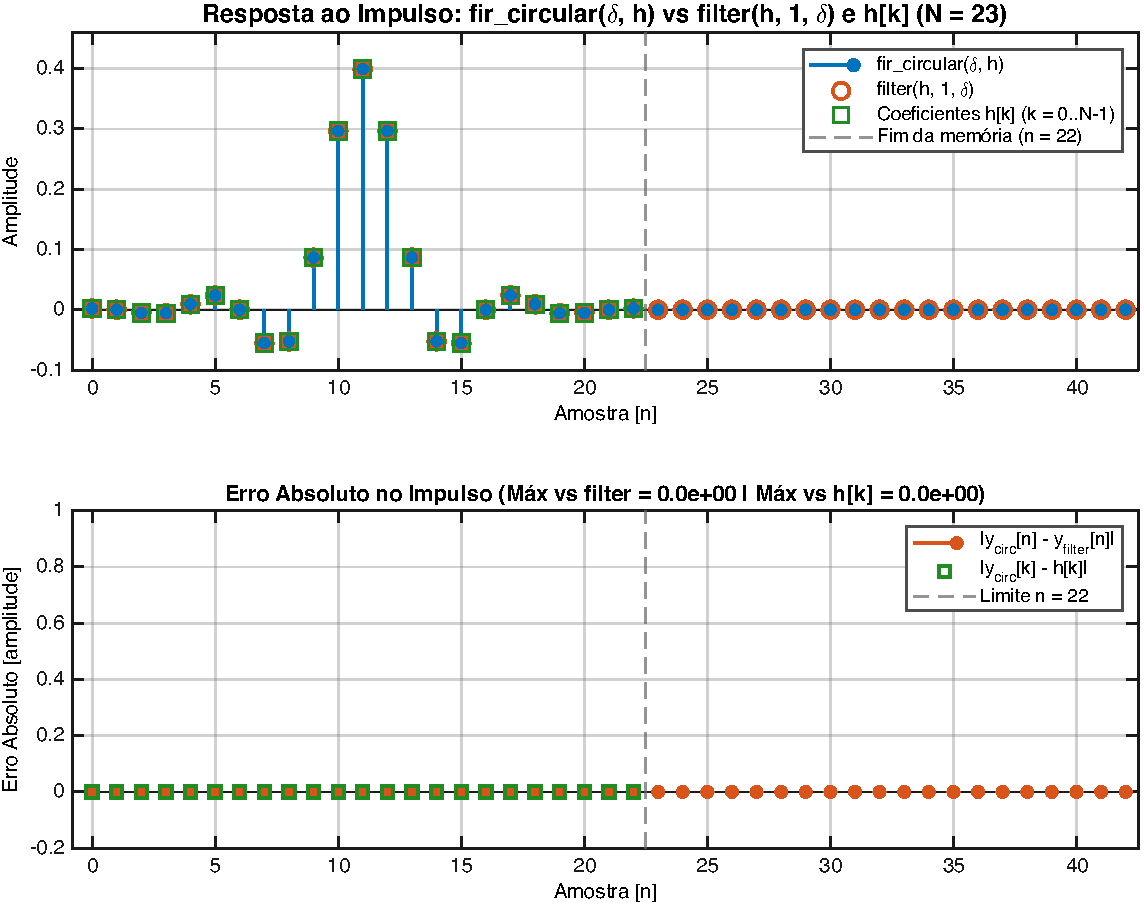
\includegraphics[width=0.92\linewidth]{fig_B1_impulso_comparacao.pdf}
    \caption{Etapa B: resposta ao impulso obtida com \texttt{fir\_circular}, comparada com os coeficientes $h[k]$ e com \texttt{filter(h,1,delta)}.}
    \label{fig:B1_impulso}
\end{figure}

\begin{figure}[H]
    \centering
    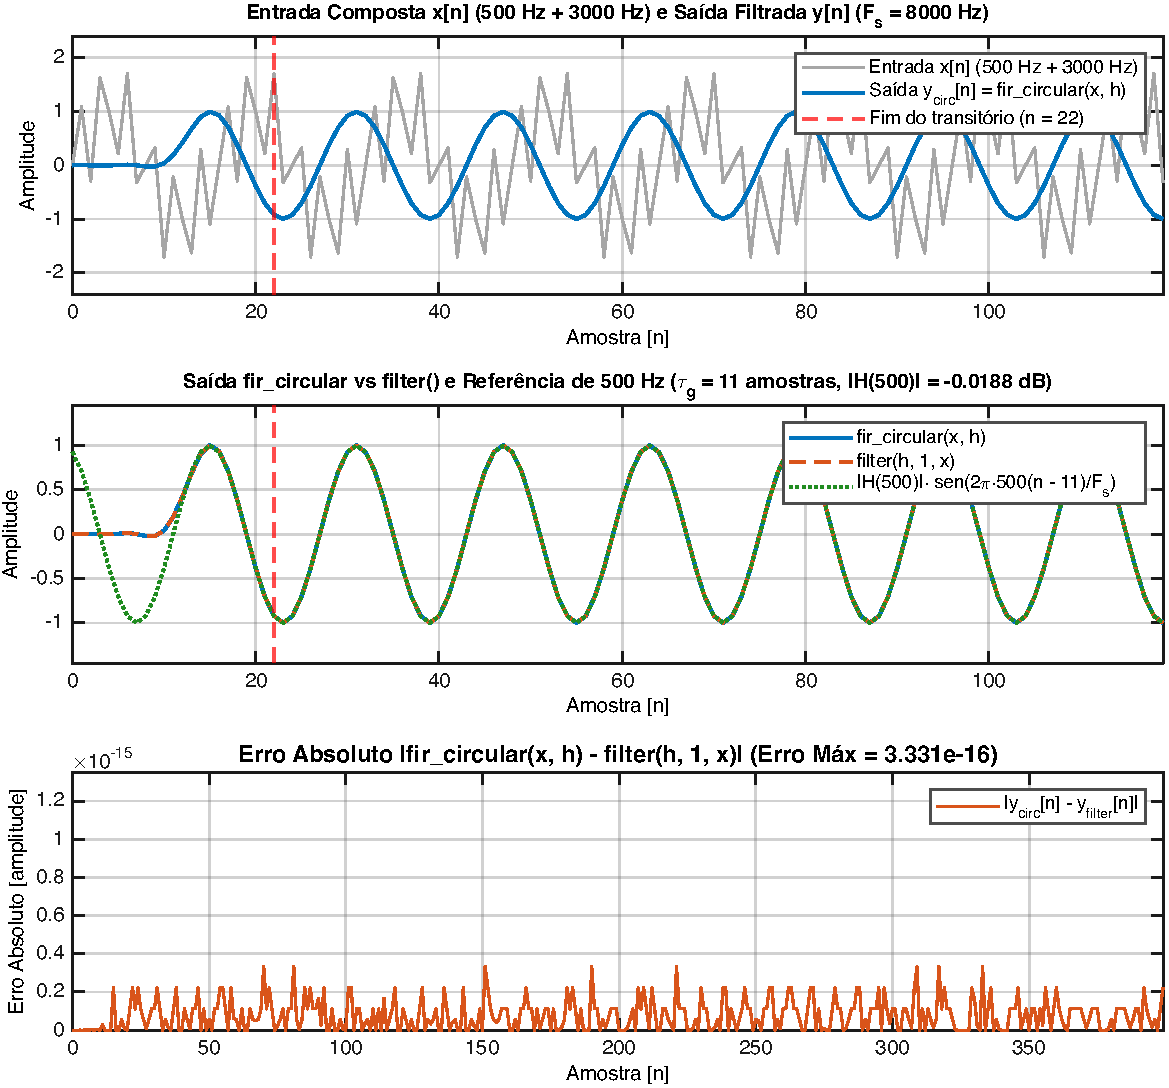
\includegraphics[width=0.95\linewidth]{fig_B2_senoides_temporal.pdf}
    \caption{Etapa B: entrada e saída para o sinal de duas senoides (\SI{500}{Hz} + \SI{3000}{Hz}): transitório de $M = 22$ amostras, rejeição da componente de \SI{3000}{Hz}, atraso de 11 amostras da componente de \SI{500}{Hz} e diferença em relação a \texttt{filter} da ordem de $10^{-16}$.}
    \label{fig:B2_senoides}
\end{figure}

\subsection{Análise (Etapa B)}

\begin{itemize}[leftmargin=1.5em, itemsep=3pt]
    \item \textbf{Por que os dados não precisam ser deslocados fisicamente.} Em uma linha de atraso linear, cada nova amostra obrigaria a mover as $M$ amostras retidas uma posição, descartando $x[n-M]$. São $M$ deslocamentos de dados por amostra, além da escrita. No buffer circular, \textbf{as amostras permanecem em suas posições na memória}: a atualização consiste apenas em mover o ponteiro uma posição no sentido anti-horário e escrever a nova amostra sobre a mais antiga, que deixou de ser necessária. O buffer circular reduz a movimentação de dados, mas \textbf{não reduz o número de multiplicações} da convolução: o filtro e sua resposta permanecem os mesmos.

    \item \textbf{Como cada coeficiente é associado à amostra correta.} Como a escrita recua uma posição (sentido anti-horário) a cada instante, a amostra escrita no instante anterior, $x[n-1]$, fica uma posição adiante no sentido horário em relação a \texttt{idx\_recente}, $x[n-2]$ fica duas posições adiante, e assim por diante. Começando a leitura em \texttt{idx\_recente} e avançando no sentido horário com retorno circular ($N \to 1$), a $k$-ésima leitura retorna $x[n-k+1]$, que é multiplicada por \texttt{h(k)} ($= b_{k-1}$). A sequência lida é $x[n] \to x[n-1] \to \cdots \to x[n-M]$, associada a $b_0, b_1, \dots, b_M$, exatamente como na Equação~\eqref{eq:fir}. Ao final da volta, o ponteiro recua e a próxima amostra é escrita na posição de $x[n-M]$.

    \item \textbf{Por que a comparação com \texttt{filter} valida a implementação, mas não substitui a verificação da máscara.} A função \texttt{filter(h,1,x)} calcula a mesma equação de diferenças para \emph{qualquer} vetor \texttt{h}. Erro nulo, ou da ordem de $10^{-16}$, prova que o buffer, os ponteiros e a acumulação estão corretos para o \texttt{h} fornecido. Essa comparação, porém, não diz nada sobre a qualidade de \texttt{h}: um vetor que não atendesse à máscara daria o mesmo erro nulo. Os ganhos em \SI{500}{Hz} e \SI{3000}{Hz} também são apenas dois pontos. A máscara só é verificada pela resposta em frequência calculada em uma grade densa de frequências, sobretudo perto das bordas \SI{1000}{Hz} e \SI{2200}{Hz}, onde $N = 22$ falhou.
\end{itemize}

% ==============================================================================
% 6. ETAPA C — QUANTIZAÇÃO DOS COEFICIENTES
% ==============================================================================
\section{Etapa C — Quantização dos Coeficientes (\texttt{Q1.15} e \texttt{Q1.7})}

\paragraph{Formato numérico.} Em ponto fixo fracionário, uma palavra de $B$ bits tem um bit de sinal e $B - 1$ bits fracionários. A resolução (passo de quantização) é dada pelo bit menos significativo: $\Delta = 2^{-F}$. Na notação do roteiro, \texttt{Q1.7} tem 8 bits (1 de sinal e $F = 7$ fracionários, $\Delta = 1/128$) e \texttt{Q1.15} tem 16 bits ($F = 15$, $\Delta = 2^{-15}$). Na notação geral $Q n.m$ da Aula~17 ($n + m = B - 1$), esses formatos correspondem a Q0.7 (\texttt{[8 7]} no MATLAB) e Q0.15, também chamado Q15 (\texttt{[16 15]}). Só podem ser representados múltiplos inteiros de $\Delta$. Por isso cada coeficiente é arredondado para o nível mais próximo:
\begin{equation}
    h_Q[k] = \frac{\operatorname{round}\!\left(h[k]\cdot 2^F\right)}{2^F}, \qquad e_Q[k] = h_Q[k] - h[k], \qquad |e_Q[k]| \le \frac{\Delta}{2}, \qquad F \in \{7,\, 15\}.
\end{equation}
Seguindo o roteiro, parte-se dos coeficientes normalizados em \texttt{double}, \textbf{não se renormaliza} após a quantização, e entradas e operações permanecem em ponto flutuante. Assim, apenas o efeito dos coeficientes é isolado. As Tabelas~\ref{tab:C1_coeficientes} e~\ref{tab:C2_metricas} e a Figura~\ref{fig:C1_quant_coef} mostram os resultados.

\begin{table}[H]
    \centering
    \caption{Coeficientes originais e quantizados, com os erros individuais $e_Q[k] = h_Q[k] - h[k]$ (\texttt{results/tab\_C1\_coeficientes\_erros.csv}).}
    \label{tab:C1_coeficientes}
    \footnotesize
    \setlength{\tabcolsep}{5pt}
    \begin{adjustbox}{max width=\textwidth}
    \begin{tabular}{@{}crrrrr@{}}
        \toprule
        \textbf{$k$} & \multicolumn{1}{c}{\textbf{$h[k]$ (\texttt{double})}} & \multicolumn{1}{c}{\textbf{$h_{\text{Q1.7}}[k]$}} & \multicolumn{1}{c}{\textbf{$e_{\text{Q1.7}}[k]$}} & \multicolumn{1}{c}{\textbf{$h_{\text{Q1.15}}[k]$}} & \multicolumn{1}{c}{\textbf{$e_{\text{Q1.15}}[k]$}} \\
        \midrule
        \rowcolor{rowfail}
        0  & $+0,00219838$ & $+0,00000000$ & $-2,198376\times 10^{-3}$ & $+0,00219727$ & $-1,110097\times 10^{-6}$ \\
        1  & $-1,5357\times 10^{-18}$ & $0,00000000$ & $+1,535651\times 10^{-18}$ & $0,00000000$ & $+1,535651\times 10^{-18}$ \\
        2  & $-0,00513949$ & $-0,00781250$ & $\mathbf{-2,673012\times 10^{-3}}$ & $-0,00512695$ & $+1,253520\times 10^{-5}$ \\
        3  & $-0,00557566$ & $-0,00781250$ & $-2,236844\times 10^{-3}$ & $-0,00558472$ & $-9,061077\times 10^{-6}$ \\
        4  & $+0,00931175$ & $+0,00781250$ & $-1,499248\times 10^{-3}$ & $+0,00930786$ & $-3,886926\times 10^{-6}$ \\
        5  & $+0,02390682$ & $+0,02343750$ & $-4,693181\times 10^{-4}$ & $+0,02389526$ & $-1,155439\times 10^{-5}$ \\
        6  & $-9,4267\times 10^{-18}$ & $0,00000000$ & $+9,426665\times 10^{-18}$ & $0,00000000$ & $+9,426665\times 10^{-18}$ \\
        7  & $-0,05524793$ & $-0,05468750$ & $+5,604296\times 10^{-4}$ & $-0,05523682$ & $+1,111321\times 10^{-5}$ \\
        8  & $-0,05238580$ & $-0,05468750$ & $-2,301705\times 10^{-3}$ & $-0,05239868$ & $-1,288655\times 10^{-5}$ \\
        9  & $+0,08658761$ & $+0,08593750$ & $-6,501124\times 10^{-4}$ & $+0,08657837$ & $-9,243257\times 10^{-6}$ \\
        10 & $+0,29664427$ & $+0,29687500$ & $+2,307295\times 10^{-4}$ & $+0,29663086$ & $-1,341114\times 10^{-5}$ \\
        \rowcolor{rowpass}
        11 & $+0,39940009$ & $+0,39843750$ & $-9,625876\times 10^{-4}$ & $+0,39941406$ & $\mathbf{+1,397490\times 10^{-5}}$ \\
        12 & $+0,29664427$ & $+0,29687500$ & $+2,307295\times 10^{-4}$ & $+0,29663086$ & $-1,341114\times 10^{-5}$ \\
        13 & $+0,08658761$ & $+0,08593750$ & $-6,501124\times 10^{-4}$ & $+0,08657837$ & $-9,243257\times 10^{-6}$ \\
        14 & $-0,05238580$ & $-0,05468750$ & $-2,301705\times 10^{-3}$ & $-0,05239868$ & $-1,288655\times 10^{-5}$ \\
        15 & $-0,05524793$ & $-0,05468750$ & $+5,604296\times 10^{-4}$ & $-0,05523682$ & $+1,111321\times 10^{-5}$ \\
        16 & $-9,4267\times 10^{-18}$ & $0,00000000$ & $+9,426665\times 10^{-18}$ & $0,00000000$ & $+9,426665\times 10^{-18}$ \\
        17 & $+0,02390682$ & $+0,02343750$ & $-4,693181\times 10^{-4}$ & $+0,02389526$ & $-1,155439\times 10^{-5}$ \\
        18 & $+0,00931175$ & $+0,00781250$ & $-1,499248\times 10^{-3}$ & $+0,00930786$ & $-3,886926\times 10^{-6}$ \\
        19 & $-0,00557566$ & $-0,00781250$ & $-2,236844\times 10^{-3}$ & $-0,00558472$ & $-9,061077\times 10^{-6}$ \\
        20 & $-0,00513949$ & $-0,00781250$ & $\mathbf{-2,673012\times 10^{-3}}$ & $-0,00512695$ & $+1,253520\times 10^{-5}$ \\
        21 & $-1,5357\times 10^{-18}$ & $0,00000000$ & $+1,535651\times 10^{-18}$ & $0,00000000$ & $+1,535651\times 10^{-18}$ \\
        \rowcolor{rowfail}
        22 & $+0,00219838$ & $+0,00000000$ & $-2,198376\times 10^{-3}$ & $+0,00219727$ & $-1,110097\times 10^{-6}$ \\
        \bottomrule
    \end{tabular}
    \end{adjustbox}
\end{table}

\begin{table}[H]
    \centering
    \caption{Erros de quantização e desempenho nas duas bandas para as três versões do filtro (\texttt{results/tab\_C2\_metricas\_quant\_coef.csv}).}
    \label{tab:C2_metricas}
    \small
    \setlength{\tabcolsep}{5pt}
    \begin{adjustbox}{max width=\textwidth}
    \begin{tabular}{@{}lccc@{}}
        \toprule
        \textbf{Grandeza} & \textbf{Original (\texttt{double})} & \textbf{\texttt{Q1.15}} & \textbf{\texttt{Q1.7}} \\
        \midrule
        Passo $\Delta = 2^{-F}$ / limite $\Delta/2$ & --- & $\num{3,051758e-5}$ / $\num{1,525879e-5}$ & $\num{7,8125e-3}$ / $\num{3,90625e-3}$ \\
        \textbf{Erro absoluto máximo} & $0$ & $\mathbf{\MetricaCErroMaxQXV}$ & $\mathbf{\MetricaCErroMaxQVII}$ \\
        \textbf{Erro quadrático médio (EQM)} & $0$ & $\mathbf{\MetricaCEQMQXV}$ & $\mathbf{\MetricaCEQMQVII}$ \\
        Coeficientes iguais a zero & --- & 4 ($k = 1, 6, 16, 21$) & 6 ($k = 0, 1, 6, 16, 21, 22$) \\
        Erro máximo de simetria & $0$ & $0$ & $0$ \\
        \textbf{Soma dos coeficientes} & $1,00000000$ & $\MetricaCSomaQXV$ & $\MetricaCSomaQVII$ ($= 125/128$) \\
        Soma dos módulos $\sum_k |h_Q[k]|$ & $\MetricaENormaLI$ & $\MetricaCSomaAbsQXV$ & $\MetricaCSomaAbsQVII$ \\
        \textbf{Ganho DC [\si{dB}]} & $0,000000$ & $\mathbf{\MetricaCGanhoDCQXVdB}$ & $\mathbf{\MetricaCGanhoDCQVIIdB}$ \\
        \textbf{Desvio máximo na passante [\si{dB}]} ($\le 0,1$) & $0,042323$ & $\mathbf{\MetricaCDesvioPassQXVdB}$ & $\mathbf{\MetricaCDesvioPassQVIIdB}$ \\
        \textbf{Atenuação mínima na rejeição [\si{dB}]} ($\ge 45$) & $47,0065$ & $\mathbf{\MetricaCAtenStopQXVdB}$ & $\mathbf{\MetricaCAtenStopQVIIdB}$ \\
        \textbf{Atende à máscara?} & \textbf{Sim} & \textbf{Sim} & \textbf{Não} (falha nas duas bandas) \\
        \bottomrule
    \end{tabular}
    \end{adjustbox}
\end{table}

\begin{figure}[H]
    \centering
    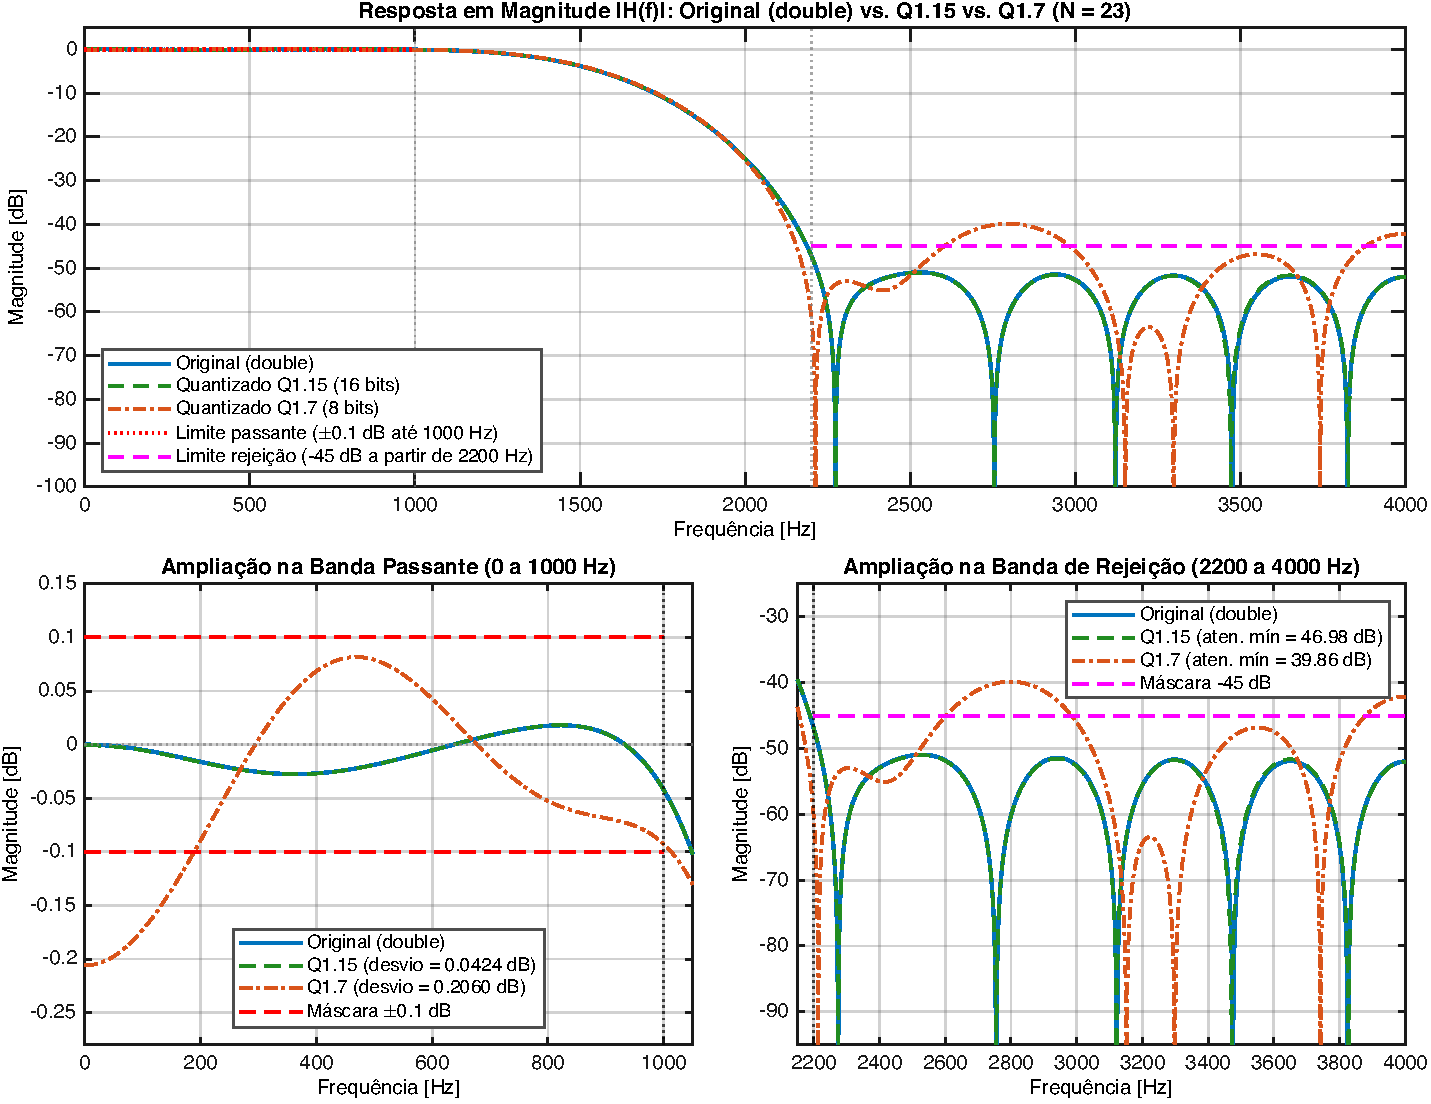
\includegraphics[width=0.96\linewidth]{fig_C1_respostas_quant_coef.pdf}
    \caption{Etapa C: magnitudes do filtro original, \texttt{Q1.15} (praticamente sobreposta à original) e \texttt{Q1.7}, de \SI{0}{Hz} a \SI{4000}{Hz}, com ampliações da passante (\SIrange{0}{1000}{Hz}) e da rejeição (\SIrange{2200}{4000}{Hz}) e os limites da máscara.}
    \label{fig:C1_quant_coef}
\end{figure}

\subsection{Questões de análise (Etapa C)}

\begin{enumerate}[leftmargin=1.6em, itemsep=3pt]
    \item \textbf{Quais coeficientes foram mais alterados?}
    Em \texttt{Q1.7}, o maior erro absoluto ocorreu no par $k = 2$ e $k = 20$: $-0,00513949 \to -1/128$, $|e| = \num{2,673012e-3}$, ou \SI{68,43}{\percent} de $\Delta/2$. Em seguida vêm os pares $k = 8, 14$ e $k = 3, 19$. Em termos relativos, os coeficientes das extremidades são os mais afetados: $h[0] = h[22]$ perdem \SI{100}{\percent} do valor, porque suas amplitudes são da mesma ordem do passo $\Delta = 1/128$. Em \texttt{Q1.15}, o maior erro ocorreu no coeficiente central $k = 11$ ($|e| = \num{1,397490e-5}$), mas ele é desprezível frente ao valor do coeficiente.

    \item \textbf{Algum foi quantizado para zero? Explique pela resolução numérica.}
    Sim. Os coeficientes $k = 1, 6, 16, 21$ já são zeros da resposta ideal: na Equação~\eqref{eq:hideal}, $0,4\,(k - 11) = \pm 2$ ou $\pm 4$, e a função $\sinc$ se anula em inteiros não nulos. Em \texttt{double}, esses coeficientes valem $\sim 10^{-18}$ e vão a zero nos dois formatos. Em \texttt{Q1.7}, \textbf{os coeficientes das extremidades $k = 0$ e $k = 22$ também foram para zero}, porque no arredondamento todo valor com $|h[k]| < \Delta/2$ cai no nível zero, e $|h[0]| = 0,00219838 < 2^{-8} = 0,00390625$. Com isso, o filtro efetivo em \texttt{Q1.7} perde as caudas da janela de Hamming. Em \texttt{Q1.15}, o limiar é $2^{-16} \approx \num{1,53e-5}$, muito menor que $h[0]$, e as caudas são preservadas.

    \item \textbf{A simetria foi preservada?}
    Sim, nas duas versões (erro de simetria nulo). Como $h[k] = h[M-k]$ antes da quantização e o arredondamento é determinístico, coeficientes iguais recebem o mesmo valor quantizado.

    \item \textbf{Qual a consequência para a fase?}
    Com a simetria preservada, as duas versões quantizadas continuam sendo filtros \textbf{tipo~I com fase linear} e atraso de grupo de $M/2 = 11$ amostras. A quantização altera apenas a amplitude real $A(\omega)$ e a posição dos zeros. Além disso, como um FIR não tem realimentação nem polos fora da origem, a quantização dos coeficientes \textbf{altera a resposta, mas não a estabilidade BIBO} (Aula~17). Esse risco existe apenas em filtros IIR com polos próximos da circunferência unitária.

    \item \textbf{Em que banda os efeitos foram mais relevantes?}
    Na \textbf{banda de rejeição}. Pela linearidade, $H_Q(e^{j\omega}) = H(e^{j\omega}) + E(e^{j\omega})$, com $E(e^{j\omega}) = \sum_k e_Q[k]\,e^{-j\omega k}$. Na rejeição, $|H|$ é muito pequeno ($\le 0,005623$), porque resulta do cancelamento entre coeficientes, e um erro da ordem de $10^{-3}$ por coeficiente basta para elevar os lóbulos laterais. Em \texttt{Q1.7}, a atenuação mínima caiu de \SI{47,0065}{dB} para \SI{39,8632}{dB}, uma perda de cerca de \SI{7,14}{dB}. Na passante, $|H| \approx 1$ é pouco sensível a erros individuais, mas em \texttt{Q1.7} os erros têm predominância negativa: sete dos nove pares não nulos e o coeficiente central foram arredondados para baixo. O resultado é um deslocamento de toda a passante para baixo (\SI{-0,205999}{dB}).

    \item \textbf{Quais versões atendem à máscara?}
    A original e a \texttt{Q1.15}: o desvio na passante passa de \SI{0,042323}{dB} para \SI{0,042440}{dB}, e a atenuação na rejeição passa de \SI{47,0065}{dB} para \SI{46,9752}{dB}. A versão \texttt{Q1.7} \textbf{falha nas duas bandas}: \SI{0,205999}{dB} $> \SI{0,1}{dB}$ e \SI{39,8632}{dB} $< \SI{45}{dB}$.

    \item \textbf{Qual a relação entre soma dos coeficientes e ganho DC?}
    O ganho DC é a própria soma: $H_Q(e^{j0}) = \sum_k h_Q[k] = 1 + \sum_k e_Q[k]$. Sem renormalização, os erros se somam em $\omega = 0$. Em \texttt{Q1.15}, a soma é \MetricaCSomaQXV{} (ganho DC de \SI{-0,000530}{dB}). Em \texttt{Q1.7}, a soma é $125/128 = 0,97656250$, e $20\log_{10}(0,9765625) = \SI{-0,205999}{dB}$, que é exatamente o pior desvio da passante. Esse resultado ilustra a conclusão da Aula~17: \textbf{a quantização pode alterar o ganho DC e a magnitude mesmo preservando a simetria e a fase linear}. A Aula~18 acrescenta que o limite de pico da saída também deve ser conferido nos coeficientes efetivamente armazenados: $\sum_k |h_Q[k]|$ vale $\MetricaCSomaAbsQXV$ em \texttt{Q1.15} e $\MetricaCSomaAbsQVII$ em \texttt{Q1.7} (Tabela~\ref{tab:C2_metricas}).

    \item \textbf{Qual precisão foi escolhida?}
    \texttt{Q1.15} (16 bits). Das duas precisões avaliadas, é a única que mantém a máscara nas duas bandas, além da simetria e da fase linear. \texttt{Q1.7} (8 bits) não é suficiente para este filtro, porque falha tanto na passante quanto na rejeição.
\end{enumerate}

% ==============================================================================
% 7. ETAPA D — QUANTIZAÇÃO DAS AMOSTRAS
% ==============================================================================
\section{Etapa D — Quantização das Amostras de Entrada em \texttt{Q1.7}}

\subsection{Procedimento}

Os coeficientes $h[k]$ foram mantidos em \texttt{double}, e apenas as amostras de entrada ($F_s = \SI{8000}{Hz}$, 800 amostras) foram quantizadas em \texttt{Q1.7} por arredondamento, com saturação ao intervalo $[-1,\; 1 - 2^{-7}]$:
\begin{equation}
    x_q[n] = \min\!\Big(\max\!\Big(\tfrac{\operatorname{round}(x[n]\cdot 2^7)}{2^7},\; -1\Big),\; 1 - 2^{-7}\Big), \qquad e[n] = x_q[n] - x[n], \qquad e_y[n] = y_q[n] - y[n].
\end{equation}
Foram usados o Caso~1, $x_1[n] = 0,8\sin(2\pi\,500n/F_s)$, e o Caso~2, $x_2[n] = 0,5\sin(2\pi\,500n/F_s) + 0,3\sin(2\pi\,3000n/F_s)$. A SNR é a razão entre as potências médias do sinal e do erro.

\paragraph{Modelo teórico (Aula~17).} Com $B = 8$ bits, o passo é $\Delta = 2^{-B+1} = 2^{-7}$. Supondo $e[n]$ aleatório e uniformemente distribuído em $[-\Delta/2,\, \Delta/2]$, a média do erro é zero e sua variância é
\begin{equation}
    \sigma_e^2 = \frac{\Delta^2}{12} = \frac{2^{-14}}{12} \approx \num{5,086e-6}, \qquad \text{SQNR} = 10\log_{10}\frac{\sigma_x^2}{\sigma_e^2},
\end{equation}
com ganho de aproximadamente \SI{6}{dB} por bit adicional. Para $\sigma_x^2 = 0,32$ (Caso~1) e $0,17$ (Caso~2), o modelo prevê \SI{47,99}{dB} e \SI{45,24}{dB}, respectivamente. Esses valores servem de referência para os valores medidos.

\paragraph{Corte do transitório na saída.} O transitório do filtro ocupa as primeiras $M = 22$ saídas. O período comum dos dois sinais é de 16 amostras ($500/8000 = 1/16$ e $3000/8000 = 3/8 = 6/16$). Por isso, descartaram-se as primeiras \textbf{32 amostras} ($\ge 22$, múltiplo de 16) e as medidas na saída usam $n = 32, \dots, 799$: 768 amostras, ou 48 períodos completos.

\begin{table}[H]
    \centering
    \caption{Quantização das amostras em \texttt{Q1.7}: erro máximo frente a $\Delta/2$, potências e SNR (\texttt{results/tab\_D1\_snr\_comparacao.csv}).}
    \label{tab:D1_snr}
    \small
    \setlength{\tabcolsep}{4.5pt}
    \begin{adjustbox}{max width=\textwidth}
    \begin{tabular}{@{}lcc@{}}
        \toprule
        \textbf{Grandeza} & \textbf{Caso 1 (\SI{500}{Hz})} & \textbf{Caso 2 (\SI{500}{Hz} + \SI{3000}{Hz})} \\
        \midrule
        Erro máximo na entrada $\max|e[n]|$ (limite $\Delta/2 = \num{3,90625e-3}$) & $\num{3,185425e-3}$ (atende) & $\num{2,776249e-3}$ (atende) \\
        Erro máximo na saída $\max|e_y[n]|$, $n \ge 32$ & $\num{1,276482e-3}$ & $\num{8,393524e-4}$ \\
        \midrule
        Potência do sinal: entrada $\rightarrow$ saída & $0,320000 \rightarrow 0,318617$ & $0,170000 \rightarrow 0,124460$ \\
        Variação da potência do sinal $\Delta P_{\text{sinal}}$ & \SI{-0,018814}{dB} & \SI{-1,354194}{dB} \\
        Potência do erro: entrada $\rightarrow$ saída & $\num{6,667355e-6} \rightarrow \num{8,304642e-7}$ & $\num{3,516992e-6} \rightarrow \num{2,110931e-7}$ \\
        Variação da potência do erro $\Delta P_{\text{ruído}}$ & \SI{-9,046327}{dB} & \SI{-12,216974}{dB} \\
        \midrule
        \textbf{SNR de entrada} & \textbf{\SI{46,8120}{dB}} & \textbf{\SI{46,8428}{dB}} \\
        \textbf{SNR de saída} & \textbf{\SI{55,8395}{dB}} & \textbf{\SI{57,7056}{dB}} \\
        \textbf{Diferença $\Delta\text{SNR}$} & \textbf{\SI{+9,0275}{dB}} & \textbf{\SI{+10,8628}{dB}} \\
        \midrule
        SQNR teórica do modelo uniforme ($\sigma_e^2 = \Delta^2/12$) & \SI{47,99}{dB} & \SI{45,24}{dB} \\
        \bottomrule
    \end{tabular}
    \end{adjustbox}
\end{table}

\begin{figure}[H]
    \centering
    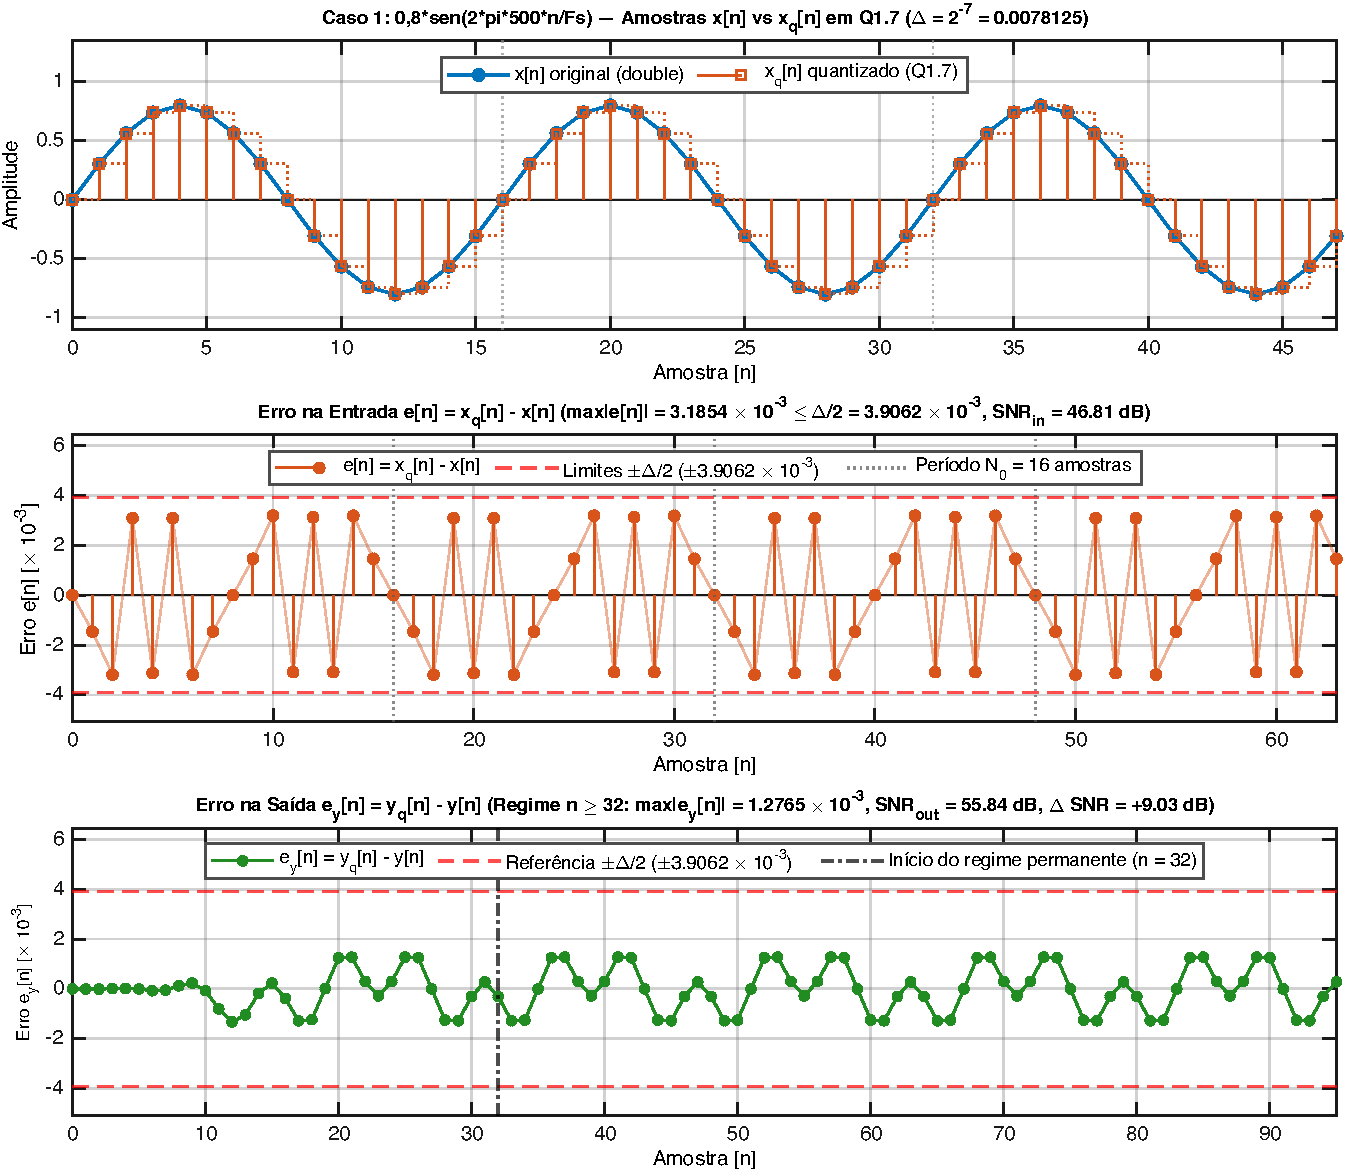
\includegraphics[width=0.95\linewidth]{fig_D1_caso1_amostras_e_erros.pdf}
    \caption{Etapa D, Caso 1: (a) amostras originais e quantizadas em \texttt{Q1.7} (marcadores evidenciam a quantização de amplitude); (b) erro na entrada $e[n]$, dentro de $\pm\Delta/2$; (c) erro na saída $e_y[n]$.}
    \label{fig:D1_caso1}
\end{figure}

\begin{figure}[H]
    \centering
    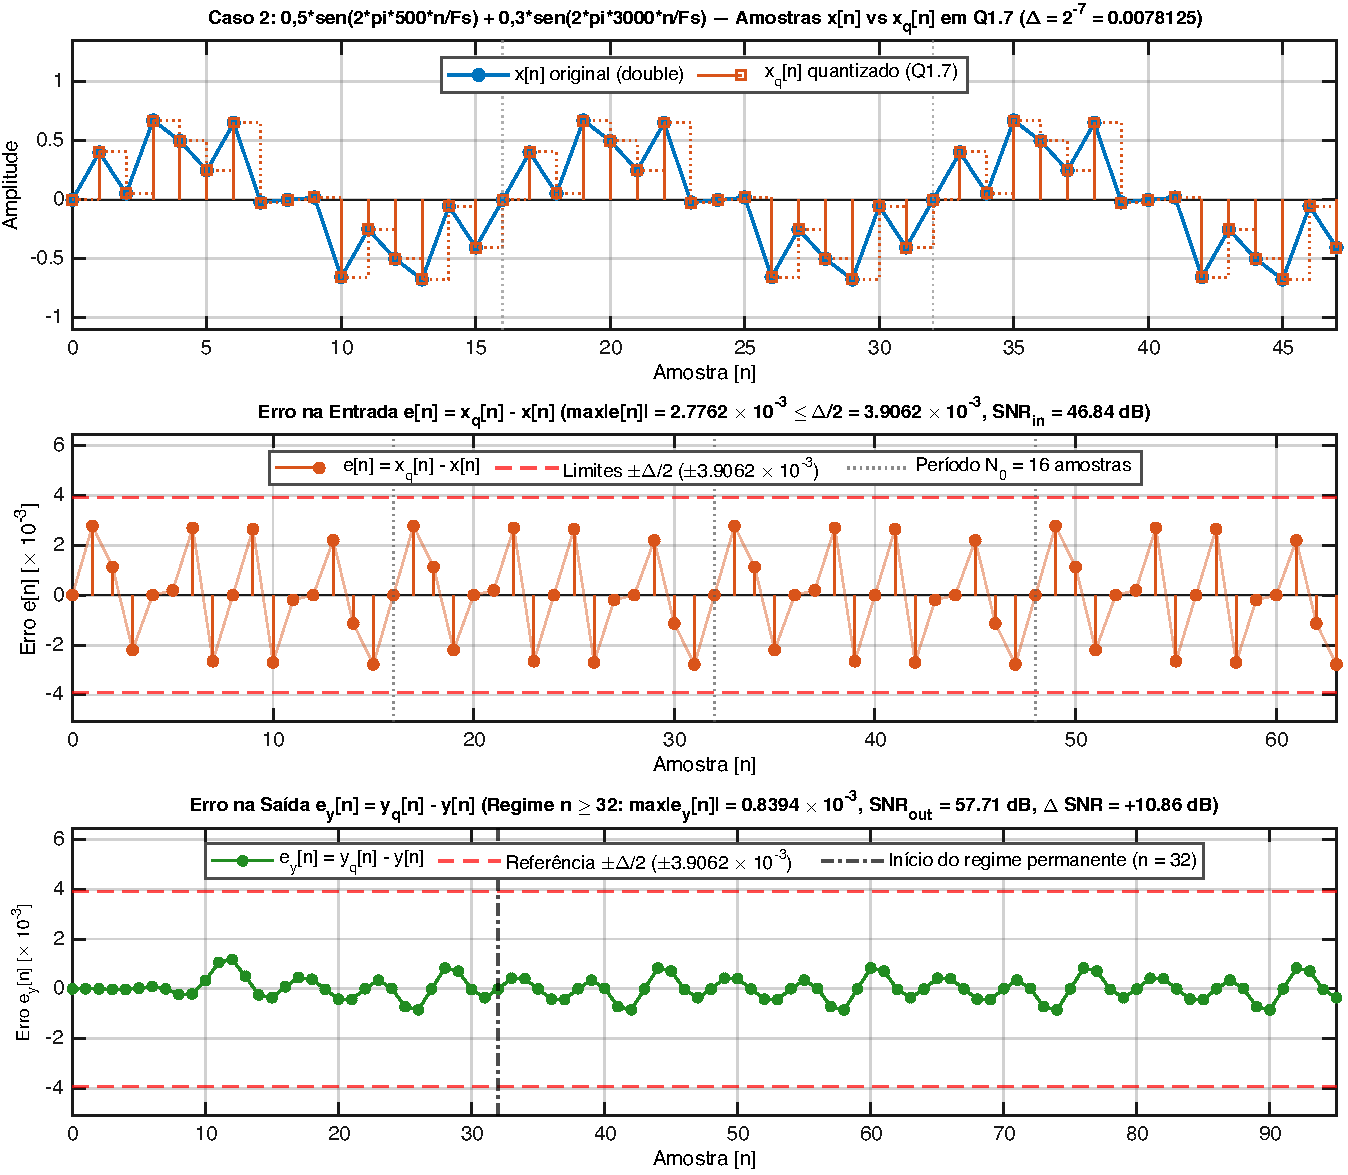
\includegraphics[width=0.95\linewidth]{fig_D2_caso2_amostras_e_erros.pdf}
    \caption{Etapa D, Caso 2: (a) amostras originais e quantizadas em \texttt{Q1.7}; (b) erro na entrada $e[n]$; (c) erro na saída $e_y[n]$.}
    \label{fig:D2_caso2}
\end{figure}

\subsection{Questões de análise (Etapa D)}

\begin{enumerate}[leftmargin=1.6em, itemsep=3pt]
    \item \textbf{O erro de quantização apresenta periodicidade? Por quê?}
    Sim, com período de 16 amostras (\SI{2}{ms}) nos dois casos, como se vê nos painéis (b) das Figuras~\ref{fig:D1_caso1} e~\ref{fig:D2_caso2}. As frequências são frações racionais de $F_s$ ($1/16$ e $3/8$), então $x[n + 16] = x[n]$. Como o quantizador é determinístico e sem memória, $x_q[n + 16] = x_q[n]$ e, portanto, $e[n + 16] = e[n]$. Assim, o erro é uma sequência periódica cuja potência fica em componentes nos múltiplos de $F_s/16 = \SI{500}{Hz}$. A hipótese de ruído aleatório e uniforme da Aula~17 não vale exatamente aqui, e isso explica por que a potência medida do erro difere de $\Delta^2/12$: ela é $1,31\times$ maior no Caso~1 e $0,69\times$ menor no Caso~2. Também por isso a SNR de entrada medida difere da SQNR teórica (Tabela~\ref{tab:D1_snr}).

    \item \textbf{Como o filtro modifica esse erro?}
    Como o filtro é linear, $y_q = h * (x + e) = y + h * e$, ou seja, $e_y[n] = (h * e)[n]$: o erro de saída é o erro de entrada filtrado pelo passa-baixa. As componentes do erro na transição e na rejeição são atenuadas, e apenas as que caem na banda passante permanecem. A potência do erro cai \SI{9,05}{dB} no Caso~1 e \SI{12,22}{dB} no Caso~2, e o pico do erro também diminui (Tabela~\ref{tab:D1_snr}).

    \item \textbf{A SNR melhora em ambos os casos?}
    Sim: \SI{+9,0275}{dB} no Caso~1 (\SI{46,8120}{dB} $\rightarrow$ \SI{55,8395}{dB}) e \SI{+10,8628}{dB} no Caso~2 (\SI{46,8428}{dB} $\rightarrow$ \SI{57,7056}{dB}).

    \item \textbf{Por que não é correto atribuir toda a variação de SNR à redução do ruído?}
    A variação de SNR se decompõe em duas parcelas:
    \begin{equation}
        \Delta\text{SNR} = 10\log_{10}\frac{P_y/P_{e_y}}{P_x/P_e} = \underbrace{10\log_{10}\frac{P_y}{P_x}}_{\Delta P_{\text{sinal}}} \;-\; \underbrace{10\log_{10}\frac{P_{e_y}}{P_e}}_{\Delta P_{\text{ruído}}}.
        \label{eq:deltasnr}
    \end{equation}
    No Caso~1, o sinal está inteiro na passante, e $\Delta P_{\text{sinal}} = \SI{-0,018814}{dB} \approx 0$: quase toda a melhora vem da redução do ruído ($-0,0188 + 9,0463 = \SI{9,0275}{dB}$). No Caso~2, o próprio sinal útil perde potência, porque a componente de \SI{3000}{Hz} (potência $0,045$, de um total de $0,170$) é rejeitada, e $\Delta P_{\text{sinal}} = \SI{-1,3542}{dB}$. Embora o ruído tenha caído \SI{12,2170}{dB}, a SNR melhorou só \SI{10,8628}{dB}. Se a maior parte da energia do sinal estivesse na rejeição, a SNR de saída poderia até piorar, mesmo com o filtro reduzindo o ruído. Por isso, é preciso analisar separadamente o que acontece com o sinal e com o ruído.
\end{enumerate}

% ==============================================================================
% 8. ETAPA E — PRECISÃO ARITMÉTICA E OVERFLOW
% ==============================================================================
\section{Etapa E — Precisão Aritmética e Overflow}

Na representação em ponto fixo, um resultado com mais bits do que o formato de destino precisa ser aproximado. No \textbf{arredondamento}, escolhe-se o nível de quantização mais próximo, com $|e| \le \Delta/2$. No \textbf{truncamento}, descartam-se os bits fracionários excedentes sem arredondar; em complemento de 2, isso equivale a \texttt{floor}, com $-\Delta < e \le 0$ e viés negativo. O exemplo usa dois operandos exatos em \texttt{Q1.7} (\texttt{src/etapa\_E\_ponto\_fixo.m}):
\begin{equation}
    a = \tfrac{79}{128} = 0,6171875, \qquad b = \tfrac{45}{128} = 0,3515625, \qquad p = a\,b = \tfrac{3555}{16384} = \MetricaEProdCompleto .
\end{equation}
O produto exato tem $7 + 7 = 14$ bits fracionários (\texttt{Q2.14}, 16 bits). Para voltar a \texttt{Q1.7}, descartam-se 7 bits, cujo valor equivale a $0,7734375$~LSB.

\begin{table}[H]
    \centering
    \caption{Etapa E: produto completo, arredondado e truncado para \texttt{Q1.7}, e exemplo de \textit{overflow} na soma (\texttt{results/tab\_E1\_produto\_Q17.csv}). LSB $= \Delta = 2^{-7}$.}
    \label{tab:E1_ponto_fixo}
    \footnotesize
    \setlength{\tabcolsep}{4.5pt}
    \begin{adjustbox}{max width=\textwidth}
    \begin{tabular}{@{}llccrr@{}}
        \toprule
        \textbf{Grandeza} & \textbf{Formato} & \textbf{Fração} & \textbf{Palavra binária} & \multicolumn{1}{c}{\textbf{Valor}} & \multicolumn{1}{c}{\textbf{Erro em relação ao exato}} \\
        \midrule
        \multicolumn{6}{@{}l}{\textbf{Parte 1 --- Produto \texttt{Q1.7} $\times$ \texttt{Q1.7}}} \\
        \midrule
        Operando $a$ & \texttt{Q1.7} & $79/128$ & \texttt{0.1001111} & $+0,6171875$ & --- \\
        Operando $b$ & \texttt{Q1.7} & $45/128$ & \texttt{0.0101101} & $+0,3515625$ & --- \\
        \textbf{Produto completo} & \textbf{\texttt{Q2.14}} & $3555/16384$ & \texttt{00.00110111100011} & $\mathbf{+0,21697998046875}$ & $0$ \\
        \rowcolor{rowpass}
        \textbf{Arredondado} (\texttt{round}) & \texttt{Q1.7} & $28/128$ & \texttt{0.0011100} & $+0,21875$ & $\mathbf{\MetricaEErroArred}$ ($+0,2265625$ LSB) \\
        \rowcolor{rowfail}
        \textbf{Truncado} (\texttt{floor}) & \texttt{Q1.7} & $27/128$ & \texttt{0.0011011} & $+0,2109375$ & $\mathbf{\MetricaEErroTrunc}$ ($-0,7734375$ LSB) \\
        \midrule
        \multicolumn{6}{@{}l}{\textbf{Parte 2 --- \textit{Overflow} na soma $0,75 + 0,50$ em \texttt{Q1.7}}} \\
        \midrule
        Soma exata & (9 bits) & $160/128$ & \texttt{01.0100000} & $+1,25$ & excede $+127/128$ \\
        \rowcolor{rowpass}
        Com \textbf{saturação} & \texttt{Q1.7} & $127/128$ & \texttt{0.1111111} & $+0,9921875$ & $-0,2578125$ \\
        \rowcolor{rowfail}
        Com \textbf{retorno circular} (\textit{wrap-around}) & \texttt{Q1.7} & $-96/128$ & \texttt{1.0100000} & $-0,75$ & $-2,0$ \\
        \bottomrule
    \end{tabular}
    \end{adjustbox}
\end{table}

No exemplo, o erro do truncamento é cerca de $3,4$ vezes maior que o do arredondamento, além de ser sempre negativo. Ao longo de muitas operações, esse viés se acumula.

\paragraph{Momento do arredondamento (Aula~18).} Na forma direta, o arredondamento pode ser feito depois de \emph{cada} multiplicação, com um bloco $Q$ em cada ramo, ou \emph{uma única vez} depois da soma final, com o acumulador guardando os produtos completos. No exemplo da aula, com dois produtos de $4,5/128$ e três produtos nulos, arredondar cada ramo dá $\MetricaEQRamo/128$, enquanto arredondar depois da soma dá o valor exato, $\MetricaEQSoma/128$. Para o filtro projetado, com $N = 23$ ramos, o erro de saída fica limitado a $N\Delta/2 = \MetricaEErroRamo$ no primeiro caso e a $\Delta/2 = \MetricaEErroSoma$ no segundo. Por isso o acumulador de um DSP é mais largo que a palavra de dados, e o arredondamento é feito só na conversão da saída.

\subsection{Questões conceituais}

\begin{enumerate}[leftmargin=1.6em, itemsep=3pt]
    \item \textbf{Por que o produto de duas palavras de 8 bits pode exigir até 16 bits, e por que a soma de produtos exige maior faixa.}
    No produto, os bits fracionários se somam ($7 + 7 = 14$) e a parte inteira também cresce. O caso extremo é $(-1) \times (-1) = +1$, que não cabe em uma palavra fracionária com apenas o bit de sinal. Por isso, o produto completo usa 16 bits (\texttt{Q2.14}). No filtro, o acumulador soma $N = 23$ produtos, e a soma pode ultrapassar a faixa $[-1, 1)$ mesmo que cada produto caiba nela. O acumulador precisa, portanto, de bits extras na parte inteira (bits de guarda). No pior caso genérico, com 23 parcelas de módulo unitário, seriam $\lceil\log_2 23\rceil = 5$ bits.

    \item \textbf{Significado da soma dos módulos dos coeficientes.}
    Para entrada limitada, $|x[n]| \le X_{\max}$, a saída obedece a
    \begin{equation}
        |y[n]| = \Big|\sum_{k=0}^{M} h[k]\,x[n-k]\Big| \le X_{\max}\sum_{k=0}^{M} |h[k]|,
    \end{equation}
    e o limite é atingido quando $x[n-k] = X_{\max}\operatorname{sgn}(h[k])$. Para o filtro projetado, $\sum_k |h[k]| = \MetricaENormaLI$ ($\MetricaENormaLIdB$~\si{dB}). Esse valor é maior que $\sum_k h[k] = 1$ por causa dos coeficientes negativos. Assim, mesmo com $|x[n]| \le 1$, a saída pode chegar a $\approx 1,47$ e ultrapassar a faixa de \texttt{Q1.7}. Basta $\lceil\log_2 1,4734\rceil = 1$ bit de guarda na saída.

    A Aula~18 transforma essa desigualdade em uma regra para a \textbf{amplitude máxima de entrada}. Se a entrada atinge $K$ passos de \texttt{Q1.7} ($|x[n]| \le K/128$), a saída pode chegar a $\sum_k|h[k]|\cdot K$ passos, e esse valor precisa caber nos 127 passos positivos de \texttt{Q1.7}. Para o filtro projetado, $K_{\max} = \MetricaEKMax$, ou seja, $|x[n]| \le \MetricaEKMax/128 = \MetricaEAMax$. Com $K_{\max}$, o pico é de $\MetricaEPicoK$ passos e cabe; com $K_{\max} + 1$, seria de $\MetricaEPicoKI$ passos e excederia 127. O limite é suficiente, mas conservador, porque só é atingido quando $x[n-k] = A\operatorname{sgn}(h[k])$. Uma senoide na banda passante, como as da Etapa~D (pico de $0,8$, processadas em \texttt{double}), sai com pico próximo de $A\,|H(f)|$.

    A alternativa é \textbf{dividir os coeficientes por $\sum_k|h[k]|$} e admitir entrada de até $127/128$. O preço é a queda do ganho DC para $\MetricaEGanhoDCEsc$ ($\MetricaEGanhoDCEscdB$~dB) antes da quantização. Além disso, os novos coeficientes precisam ser arredondados para \texttt{Q1.7}, e a verificação final deve usar os valores armazenados. Para este filtro, $\sum_k|h_q[k]| = \MetricaESomaAbsEscQInt/128 = \MetricaESomaAbsEscQ$ e $\sum_k h_q[k] = \MetricaESomaEscQInt/128 = \MetricaESomaEscQ$ ($\MetricaEGanhoDCEscQdB$~dB). Como $\sum_k|h_q[k]| > 1$, o pior caso com entrada $127/128$ chega a $\MetricaEPicoEscQ$ e ainda excede $127/128$: o arredondamento desfez parte do escalonamento. É por isso que a aula recomenda conferir \texttt{sum(abs(hq))}, \texttt{sum(hq)} e \texttt{freqz(hq,1,...)} depois da quantização.

    \item \textbf{\textit{Overflow}, saturação e retorno circular.}
    Ocorre \textit{overflow} quando o resultado excede a faixa representável do formato de destino (em \texttt{Q1.7}, de $-1$ a $+127/128$). Na \textbf{saturação}, o resultado é limitado ao extremo de mesmo sinal: $0,75 + 0,50 \to +127/128$. O erro é limitado ($0,2578$) e a polaridade é preservada. No \textbf{retorno circular}, que é o comportamento natural do complemento de 2 quando o vai-um para o bit de sinal é ignorado, $01100000_2 + 01000000_2 = 10100000_2$. O acumulador guardaria a soma exata em 9 bits, \texttt{01.0100000}; ao conservar só os 8 bits da direita, sobra \texttt{1.0100000}. Como em complemento de 2 o bit à esquerda da vírgula tem \textbf{peso $-1$} em \texttt{Q1.7} (Aula~18), essa palavra vale $-1 + 1/4 = -0,75$. O sinal inverte e o erro ($2,0$) vale toda a faixa, por isso o retorno circular é muito mais prejudicial ao sinal filtrado.
\end{enumerate}

% ==============================================================================
% 9. CONCLUSÃO TÉCNICA
% ==============================================================================
\section{Conclusão Técnica}

\begin{enumerate}[label=\textbf{(\roman*)}, leftmargin=2.2em, itemsep=5pt]
    \item \textbf{Projeto e máscara.} O método da série de Fourier com janela de Hamming e normalização da soma produziu um FIR tipo~I com fase linear e atraso de grupo constante de $M/2 = 11$ amostras (\SI{1,375}{ms}). A estimativa $N \approx 3,3/(\Delta f/F_s) = 22$ foi apenas o ponto de partida: $N = 21$ e $N = 22$ falharam na rejeição. O menor comprimento testado que atende à máscara foi $\mathbf{N = 23}$ ($M = 22$), com desvio na passante de \SI{0,042323}{dB} e atenuação mínima de \SI{47,0065}{dB}. Como referência, o \textit{Equiripple} de ordem mínima, que distribui o erro uniformemente pelas bandas, atende à mesma máscara com 15 coeficientes, o que reduz em \SI{34,78}{\percent} as multiplicações por amostra na forma direta.

    \item \textbf{Correção funcional do buffer circular.} A função \texttt{fir\_circular}, com escrita no sentido anti-horário sobre a amostra mais antiga e leitura horária a partir da mais recente, reproduziu \texttt{filter(h,1,x)} com erro nulo no impulso e de $\num{3,330669e-16}$ no sinal de duas senoides, sem deslocar dados na memória. Essa comparação valida a implementação; a máscara foi verificada separadamente pela resposta em frequência.

    \item \textbf{Quantização dos coeficientes.} O arredondamento sem renormalização preservou a simetria e, portanto, a fase linear, e não afeta a estabilidade do FIR. Em \texttt{Q1.15}, a resposta praticamente não mudou e o filtro continua atendendo à máscara. Em \texttt{Q1.7}, o passo $1/128$ zerou os coeficientes das extremidades e reduziu a soma dos coeficientes para $125/128$. O filtro falhou nas duas bandas: atenuação de \SI{39,8632}{dB} e deslocamento da passante (e do ganho DC) para \SI{-0,205999}{dB}. A banda de rejeição foi a mais sensível. Por isso, a precisão adotada para os coeficientes é \texttt{Q1.15}.

    \item \textbf{Quantização das amostras.} Em \texttt{Q1.7}, o erro de entrada respeitou o limite $\pm\Delta/2$ e foi periódico (16 amostras), pois as senoides são comensuráveis com $F_s$. Por isso, o modelo de ruído uniforme ($\Delta^2/12$) é só uma aproximação nesse caso. O filtro reduziu a potência do erro, e a SNR subiu \SI{9,03}{dB} no Caso~1 e \SI{10,86}{dB} no Caso~2. No Caso~2, parte da variação de SNR vem da queda da potência do próprio sinal (\SI{-1,35}{dB}), então a melhora não pode ser atribuída apenas à redução do ruído.

    \item \textbf{Limites da aritmética finita.} O produto de dois operandos \texttt{Q1.7} exige 16 bits para ser preservado, e a soma de $N$ produtos exige bits de guarda. Ao reduzir o produto para \texttt{Q1.7}, o arredondamento produziu erro menor e sem viés ($+0,227$ LSB) do que o truncamento ($-0,773$ LSB). Arredondar uma única vez depois da soma limita o erro a $\Delta/2$, contra $N\Delta/2$ com arredondamento em cada ramo. A soma dos módulos dos coeficientes ($\approx 1,47$) mostra que a saída pode exceder a faixa unitária mesmo com entrada limitada, o que justifica bits de guarda ou entrada limitada a $\MetricaEKMax/128$. Dividir os coeficientes por essa soma reduz o ganho DC e, depois da quantização em \texttt{Q1.7}, ainda deixa $\sum_k|h_q[k]| > 1$, então a verificação precisa usar os coeficientes armazenados. Havendo \textit{overflow}, a saturação é preferível ao retorno circular, que inverte o sinal do resultado.
\end{enumerate}

% ==============================================================================
% REFERÊNCIAS
% ==============================================================================
\section*{Referências}
\begin{itemize}[leftmargin=1.5em, itemsep=1pt]
    \item SARNO FILHO, E. P. \textit{Processamento Digital de Sinais} --- Aulas 12 a 18 (Filtros digitais; Filtros FIR de fase linear, partes 1 a 3; Implementação FIR; Quantização em filtros FIR, partes 1 e 2). SENAI CIMATEC, 2026.
    \item SARNO FILHO, E. P. \textit{Roteiro da Prática 3 --- Projeto de Filtro FIR Passa-Baixa}. SENAI CIMATEC, 2026.
    \item DINIZ, P. S. R.; DA SILVA, E. A. B.; NETTO, S. L. \textit{Processamento digital de sinais: projeto e análise de sistemas}. Bookman, 2014.
    \item LYONS, R. G. \textit{Understanding Digital Signal Processing}. Wiley, 2012.
    \item MANOLAKIS, D. G.; INGLE, V. K. \textit{Applied Digital Signal Processing: Theory and Practice}. Cambridge University Press, 2015.
    \item OPPENHEIM, A. V. \textit{Discrete-Time Signal Processing}. Pearson, 2011.
\end{itemize}

\end{document}
